% !TeX program = xelatex
% Proposal Tesis — kompilasi: latexmk -xelatex -bibtex main.tex  (atau: make)
\documentclass[12pt,a4paper]{report}

% Format ITB (font, margin, penomoran, daftar isi) ada di ../common/itb-tesis.sty
% agar proposal dan laporan akhir memakai gaya yang persis sama.
\usepackage{../common/itb-tesis}

\begin{document}

% Mengatur jarak antarbaris menjadi 1,5 spasi.
\onehalfspacing

% ==========================================
% SAMPUL
% ==========================================
\begin{titlepage}
    \centering
    \vspace*{1cm}
    
    {\fontsize{14pt}{16pt}\selectfont\bfseries
    IMPLEMENTASI FISIK DAN EVALUASI \textit{EVENT-BASED RECONFIGURATION CONTROL} PADA SISTEM FORMASI ADAPTIF TERDESENTRALISASI KAWANAN \textit{QUADCOPTER} DI RUANG SEMPIT\par}
    
    \vspace{2.0cm}
    {\large \bfseries PROPOSAL TESIS\par}
    \vspace{1.5cm}
    
    
\includegraphics[width=3cm]{logo_itb.png}\par
    
    \vspace{1.5cm}
    Oleh\par
    \vspace{0.5cm}
    {\large \bfseries Izma Alhazmi Herdian}\par
    {\large \bfseries 23825301}\par
    
    \vfill
    
    {\large \bfseries 
    MAGISTER INSTRUMENTASI DAN KONTROL\par
    FAKULTAS TEKNOLOGI INDUSTRI\par
    INSTITUT TEKNOLOGI BANDUNG\par
    2026\par}
\end{titlepage}

% Penomoran romawi untuk halaman depan
\pagenumbering{roman}
\setcounter{page}{1}

% ==========================================
% ABSTRAK
% ==========================================
\chapter*{ABSTRAK}
\addcontentsline{toc}{chapter}{ABSTRAK}

\begin{center}
    \textbf{IMPLEMENTASI FISIK DAN EVALUASI \textit{EVENT-BASED RECONFIGURATION CONTROL} PADA SISTEM FORMASI ADAPTIF TERDESENTRALISASI KAWANAN \textit{QUADCOPTER} DI RUANG SEMPIT}

    \vspace{0.8cm}
    Oleh\\
    \textbf{Izma Alhazmi Herdian}\\
    23825301

    \vspace{0.8cm}
    (Program Studi Instrumentasi dan Kontrol)
\end{center}

\vspace{0.8cm}

\noindent
Navigasi kawanan \textit{quadcopter} di ruang sempit membutuhkan sistem kontrol formasi yang adaptif sekaligus efisien dalam pertukaran data komunikasi. Penelitian ini mengimplementasikan dan mengevaluasi sistem kontrol desentralisasi formasi adaptif menggunakan \textit{Event-Based Reconfiguration Control} (ERC) yang dipadukan dengan \textit{Improved Artificial Potential Field} (IAPF) pada platform perangkat keras fisik lima unit \textit{quadcopter cinewhoop}. Setiap agen mengestimasi ketersediaan ruang secara mandiri menggunakan sensor jarak lateral dan melakukan rekonfigurasi otonom saat menghadapi penyempitan celah di koridor uji. Melalui mekanisme berbasis kejadian, paket komunikasi antar-agen hanya ditransmisikan saat parameter persepsi lingkungan melewati ambang batas tertentu, sehingga konsumsi \textit{bandwidth} jaringan dapat direduksi secara signifikan dibandingkan skema komunikasi periodik konvensional.

\noindent
Evaluasi eksperimental difokuskan pada keberhasilan transisi formasi, akurasi pelacakan lintasan, efisiensi lalu lintas data nirkabel, dan ketahanan sistem terhadap kendala fisik dunia nyata, khususnya latensi komunikasi UDP lokal dan derau sensor lokalisasi kamera atas berbasis \textit{AprilTag}. Hasil penelitian ini diharapkan dapat memberikan validasi empiris atas kinerja algoritma ERC pada perangkat keras tertanam, menghasilkan rancangan sistem kontrol multi-agen yang terukur, tangguh, dan aplikatif untuk navigasi ruang terbatas di dunia nyata.

\vspace{1cm}
\noindent \textbf{Kata kunci:} quadcopter, kontrol desentralisasi, formasi adaptif, \textit{event-based reconfiguration control}, navigasi kawanan, ruang sempit.

% ==========================================
% ABSTRACT
% ==========================================
\chapter*{ABSTRACT}
\addcontentsline{toc}{chapter}{ABSTRACT}

\begin{center}
    \textbf{PHYSICAL IMPLEMENTATION AND EVALUATION OF \textit{EVENT-BASED RECONFIGURATION CONTROL} FOR DECENTRALIZED ADAPTIVE FORMATION OF QUADCOPTER SWARMS IN NARROW SPACES}

    \vspace{0.8cm}
    By\\
    \textbf{Izma Alhazmi Herdian}\\
    23825301

    \vspace{0.8cm}
    (Instrumentation and Control Study Program)
\end{center}

\vspace{0.8cm}

\noindent
Autonomous quadcopter swarm navigation in confined environments requires an adaptive formation control system that is computationally and communicationally efficient. This research implements and evaluates a decentralized adaptive formation control system using \textit{Event-Based Reconfiguration Control} (ERC) coupled with \textit{Improved Artificial Potential Field} (IAPF) on physical hardware comprising five cinewhoop quadcopters. Each agent independently perceives spatial constraints using onboard lateral distance sensors and executes autonomous reconfiguration when traversing narrow bottlenecks in an indoor testing corridor. Through the event-triggered mechanism, inter-agent communication packets are broadcast only when environmental perception parameters cross predefined thresholds, significantly reducing network bandwidth consumption compared to conventional time-triggered periodic transmission schemes.

\noindent
The experimental evaluation focuses on formation transition success, trajectory tracking accuracy, wireless communication efficiency, and system robustness against real-world physical constraints, specifically local UDP wireless communication latency and AprilTag-based overhead camera localization noise. This study aims to provide empirical validation of the ERC algorithm on embedded hardware, establishing a scalable, robust, and deployable multi-agent control architecture for confined-space navigation.

\vspace{1cm}
\noindent \textbf{Keywords:} quadcopter, decentralized control, adaptive formation, \textit{event-based reconfiguration control}, swarm navigation, confined spaces.

% ==========================================
% HALAMAN PENGESAHAN
% ==========================================
\chapter*{HALAMAN PENGESAHAN}
\addcontentsline{toc}{chapter}{HALAMAN PENGESAHAN}

\begin{center}
    \textbf{IMPLEMENTASI FISIK DAN EVALUASI \textit{EVENT-BASED RECONFIGURATION CONTROL} PADA SISTEM FORMASI ADAPTIF TERDESENTRALISASI KAWANAN \textit{QUADCOPTER} DI RUANG SEMPIT}

    \vspace{0.8cm}
    Oleh\\
    \textbf{Izma Alhazmi Herdian}\\
    NIM: 23825301

    \vspace{0.8cm}
    (Program Studi Instrumentasi dan Kontrol)

    \vspace{0.8cm}
    Institut Teknologi Bandung

    \vspace{1.5cm}
    Menyetujui\\
    Tim Pembimbing

    \vspace{0.8cm}
    Tanggal 17 Agustus 2026
\end{center}

\vspace{1.2cm}

\noindent
\begin{minipage}[t]{0.49\textwidth}
    \centering
    Pembimbing 1

    \vspace{2.5cm}

    {\bfseries Ir. Estiyanti Ekawati, M.T., Ph.D.}\\
    NIP. 19690805 200801 2 020
\end{minipage}
\hfill
\begin{minipage}[t]{0.49\textwidth}
    \centering
    Pembimbing 2

    \vspace{2.5cm}

    {\bfseries Faqihza Mukhlish, S.T., M.T., Ph.D.}\\
    NIP. 121110001 
\end{minipage}

% ==========================================
% KATA PENGANTAR
% ==========================================
\chapter*{KATA PENGANTAR}
\addcontentsline{toc}{chapter}{KATA PENGANTAR}

Segala puji dan syukur penulis panjatkan ke hadirat Allah Swt. atas rahmat dan hidayah-Nya, sehingga penulis dapat menyelesaikan proposal tesis yang berjudul ``Implementasi Fisik dan Evaluasi \textit{Event-Based Reconfiguration Control} pada Sistem Formasi Adaptif Terdesentralisasi Kawanan \textit{Quadcopter} di Ruang Sempit''. Proposal tesis ini disusun sebagai bagian dari pemenuhan syarat akademik untuk memperoleh gelar Magister di Program Studi Instrumentasi dan Kontrol, Fakultas Teknologi Industri, Institut Teknologi Bandung. Penulis berharap bahwa proposal ini dapat menjadi landasan dalam perancangan sistem kontrol desentralisasi formasi adaptif untuk navigasi kawanan quadcopter serta memberikan referensi bagi pengembangan lebih lanjut di bidang terkait.

Penulis menyadari sepenuhnya bahwa penyusunan proposal tesis ini tidak mungkin terwujud tanpa bimbingan, dukungan, dan bantuan dari berbagai pihak. Oleh karena itu, penghargaan dan rasa terima kasih yang sebesar-besarnya disampaikan kepada:

\begin{enumerate}
    \item Ir. Estiyanti Ekawati, M.T., Ph.D., selaku dosen pembimbing pertama yang telah memberikan bimbingan, arahan, masukan teknis, serta metodologi penelitian yang sangat berharga selama proses pengerjaan tesis ini.
    \item Faqihza Mukhlish, S.T., M.T., Ph.D., selaku dosen pembimbing kedua yang telah memberikan bimbingan, arahan, masukan, serta bantuan dalam memecahkan permasalahan teknis yang dihadapi selama penelitian.
    \item Seluruh dosen dan tenaga kependidikan di Program Studi Instrumentasi dan Kontrol, atas dukungan dalam berbagai aspek akademik serta bantuan dalam hal administratif.
    \item Rekan-rekan di Pusat Teknologi, Instrumentasi, dan Otomasi, atas dukungan, diskusi, dan pertukaran gagasan selama proses penelitian.
    \item Kedua orang tua penulis yang senantiasa memberikan doa, semangat, serta dukungan moral, materiil, dan motivasi yang tiada henti.
    \item Seluruh pihak yang telah membantu dalam berbagai bentuk, baik secara langsung maupun tidak langsung, yang tidak dapat disebutkan satu per satu.
\end{enumerate}

Penulisan proposal ini masih jauh dari kesempurnaan dan memiliki berbagai keterbatasan, baik dalam hal substansi maupun penyajiannya. Oleh karena itu, penulis sangat mengharapkan kritik dan saran yang membangun agar proposal ini dapat disempurnakan serta menjadi lebih baik di masa mendatang.

\vspace{1cm}
\begin{flushright}
    Bandung, 17 Agustus 2026\\[1.8cm]
    Penulis
\end{flushright}

% ==========================================
% DAFTAR ISI, GAMBAR, TABEL, SINGKATAN
% ==========================================
\clearpage
\tableofcontents
\clearpage

\clearpage
\addcontentsline{toc}{chapter}{DAFTAR GAMBAR}
\listoffigures
\clearpage

\clearpage
\addcontentsline{toc}{chapter}{DAFTAR TABEL}
\listoftables
\clearpage

\chapter*{DAFTAR SINGKATAN DAN LAMBANG}
\addcontentsline{toc}{chapter}{DAFTAR SINGKATAN DAN LAMBANG}

\noindent
Daftar singkatan dan lambang yang digunakan dalam proposal ini disusun secara alfabetis untuk memudahkan pembaca dalam memahami istilah teknis, variabel, dan parameter yang muncul pada pembahasan.

\vspace{0.5cm}
\noindent\textbf{Daftar Singkatan}

\vspace{0.3cm}
\noindent\begin{tabularx}{\textwidth}{|>{\bfseries}p{2.4cm}|X|>{\centering\arraybackslash}p{1.8cm}|}
    \hline
    \rowcolor{gray!20}
    \thead{Singkatan} & \thead{Keterangan} & \thead{Hal.} \\ \hline
    CC & \textit{Companion Computer} & \pageref{abbr:cc} \\ \hline
    EKF & \textit{Extended Kalman Filter} & \pageref{abbr:ekf} \\ \hline
    ERC & \textit{Event-Based Reconfiguration Control} & \pageref{abbr:erc} \\ \hline
    ESC & \textit{Electronic Speed Controller} & \pageref{abbr:esc} \\ \hline
    FC & \textit{Flight Controller} & \pageref{abbr:fc} \\ \hline
    HITL & \textit{Hardware-In-The-Loop} & \pageref{abbr:hitl} \\ \hline
    IAPF & \textit{Improved Artificial Potential Field} & \pageref{abbr:iapf} \\ \hline
    MAVLink & \textit{Micro Air Vehicle Link} & \pageref{abbr:mavlink} \\ \hline
    PID & \textit{Proportional-Integral-Derivative} & \pageref{abbr:pid} \\ \hline
    PTIO & Pusat Teknologi Instrumentasi dan Otomasi & \pageref{abbr:ptio} \\ \hline
    RAB & Rencana Anggaran Biaya & \pageref{abbr:rab} \\ \hline
    RMSE & \textit{Root Mean Square Error} & \pageref{abbr:rmse} \\ \hline
    UAV & \textit{Unmanned Aerial Vehicle} & \pageref{abbr:uav} \\ \hline
    UDP & \textit{User Datagram Protocol} & \pageref{abbr:udp} \\ \hline
\end{tabularx}

\clearpage
\noindent\textbf{Daftar Lambang}

\vspace{0.3cm}
\noindent\begin{tabularx}{\textwidth}{|>{\centering\arraybackslash\bfseries}p{3cm}|X|>{\centering\arraybackslash}p{1.8cm}|}
    \hline
    \rowcolor{gray!20}
    \thead{Lambang} & \thead{Keterangan} & \thead{Hal.} \\ \hline
    $d_l$ & Jarak lateral antara sisi kiri wahana dan dinding atau rintangan kiri. & \pageref{sym:dl} \\ \hline
    $d_r$ & Jarak lateral antara sisi kanan wahana dan dinding atau rintangan kanan. & \pageref{sym:dr} \\ \hline
    $\phi$ (\textit{phi}) & Sudut rotasi \textit{roll} pada dinamika \textit{quadcopter}. & \pageref{sym:phi} \\ \hline
    $\psi$ (\textit{psi}) & Sudut rotasi \textit{yaw} pada dinamika \textit{quadcopter}. & \pageref{sym:psi} \\ \hline
    $\theta$ (\textit{theta}) & Sudut rotasi \textit{pitch} pada dinamika \textit{quadcopter}. & \pageref{sym:theta} \\ \hline
    $w_{\mathrm{body}}$ & Lebar fisik badan wahana quadcopter. & \pageref{sym:wbody} \\ \hline
    $w_e$ & Estimasi lebar ruang atau celah yang dihitung dari jarak lateral dan lebar badan wahana. & \pageref{sym:we} \\ \hline
    $x$ & Sumbu posisi longitudinal pada ruang tiga dimensi. & \pageref{sym:x} \\ \hline
    $y$ & Sumbu posisi lateral pada ruang tiga dimensi. & \pageref{sym:y} \\ \hline
    $z$ & Sumbu posisi vertikal pada ruang tiga dimensi. & \pageref{sym:z} \\ \hline
\end{tabularx}

\clearpage

% Penomoran arab untuk konten utama
\pagenumbering{arabic}
\setcounter{page}{1}

% ==========================================
% BAB I PENDAHULUAN
% ==========================================
\chapter{PENDAHULUAN}

\section{Latar Belakang}
Navigasi terkoordinasi kawanan wahana udara tak berawak (\textit{Unmanned Aerial Vehicle}/UAV\label{abbr:uav}) jenis \textit{quadcopter} di ruang sempit menuntut sistem kontrol formasi yang adaptif sekaligus efisien dalam pertukaran data komunikasi \cite{gettinger3DefiningDrones2024}. Pada sistem multi-agen ini, setiap wahana bergerak dalam ruang tiga dimensi pada koordinat posisi $x$\label{sym:x}, $y$\label{sym:y}, dan $z$\label{sym:z}, dengan orientasi sikap bodi yang dinyatakan oleh sudut \textit{roll} ($\phi$\label{sym:phi}), \textit{pitch} ($\theta$\label{sym:theta}), dan \textit{yaw} ($\psi$\label{sym:psi}) \cite{brescianiniNonlinearQuadrocopterAttitude2013a, johnBobzwikQuadcopter_SimCon2025}. Masing-masing \textit{quadcopter} dituntut untuk mempertahankan kestabilan sikap dan posisi sekaligus menyesuaikan jarak relatif terhadap agen lain dan rintangan lingkungan secara dinamis \cite{kurochkinMethodsFormationControl2021}. Sistem kawanan ini membuka keunggulan operasional yang signifikan untuk misi penjelajahan area sempit, pencarian korban bencana \cite{dealcantaraandradeAutonomousUnmannedAerial2019}, inspeksi infrastruktur \cite{sanchez-cuevasFullyActuatedAerialManipulator2020}, serta patroli keamanan terdistribusi \cite{borkarReconfigurableFormationsQuadrotors2020}.

Tantangan mendasar pada navigasi kawanan di ruang sempit adalah menjaga geometri formasi tanpa mengorbankan keselamatan navigasi. Ketika melewati celah sempit, formasi geometri kaku (seperti formasi V atau segitiga) tidak dapat dipertahankan dan harus bertransisi secara otonom menjadi konfigurasi ramping (seperti formasi berbaris atau mengekor). Berbagai pendekatan kontrol formasi telah dikembangkan dalam literatur, meliputi \textit{leader-follower} \cite{abroComprehensiveReviewNextGen2025}, \textit{virtual structure} \cite{renFormationFeedbackControl2004, liuDecentralizationVirtualLinkage2018}, dan \textit{behavior-based} \cite{balchBehaviorbasedFormationControl1998}. Untuk penghindaran rintangan, metode \textit{Artificial Potential Field} (APF) banyak diterapkan dan disempurnakan menjadi \textit{Improved Artificial Potential Field} (IAPF) guna mengatasi jebakan minimum lokal \cite{wangUAVFormationObstacle2021, buiEventbasedReconfigurationControl2025}. Lebih lanjut, strategi \textit{Event-Based Reconfiguration Control} (ERC\label{abbr:erc}) diperkenalkan untuk memungkinkan adaptasi konfigurasi formasi yang dipicu hanya ketika parameter persepsi lingkungan melewati ambang batas toleransi tertentu \cite{buiEventbasedReconfigurationControl2025}. Mekanisme berbasis kejadian ini secara teoretis mampu mereduksi pertukaran data komunikasi antar-agen dibandingkan skema periodik konvensional.

Meskipun algoritma desentralisasi berbasis ERC dan IAPF telah terbukti efektif dalam lingkungan simulasi numerik, penerapannya pada platform perangkat keras fisik menghadirkan kesenjangan realitas yang kompleks. Pada wahana fisik, keandalan sistem multi-agen dibatasi oleh ketidaksempurnaan dinamika dunia nyata, meliputi latensi transmisi jaringan nirkabel \cite{chenReviewUnmannedAerial2020}, keterbatasan \textit{bandwidth} komunikasi \cite{baktayanComputationalOffloadingUAV2024}, derau sensor lokalisasi dalam ruangan \cite{georgiadisReviewLocalizationSensing2025, liuSurveySensorsBased2025}, serta kapasitas komputasi \textit{companion computer} pada wahana \cite{ahmedSurveyUAVComputing2022}. Sebagian besar studi perangkat keras kawanan quadcopter saat ini masih mengandalkan arsitektur kontrol terpusat atau menyederhanakan skenario navigasi untuk menghindari instabilitas komputasi \cite{alqudsiUAVSwarmsResearch2025}. Validasi empiris terhadap keandalan mekanisme pemicu kejadian ERC pada sistem fisik terdesentralisasi penuh di ruang sempit masih sangat terbatas dalam literatur terkini.

Pada penelitian pendahuluan, sistem kontrol dan navigasi kawanan \textit{quadcopter} telah dimodelkan dan divalidasi pada simulator komputasional, di mana kombinasi IAPF dan ERC terbukti mampu mempertahankan formasi serta mengeksekusi rekonfigurasi bentuk saat melintasi celah lorong sempit \cite{herdianDecentralizedFormationControl2026}. Membangun di atas fondasi hasil simulasi tersebut, penelitian tesis ini difokuskan untuk menjembatani kesenjangan antara model teoretis dan platform fisik di dunia nyata. Tesis ini merealisasikan, menguji, dan mengevaluasi kinerja sistem kontrol formasi adaptif terdesentralisasi menggunakan algoritma ERC secara langsung pada lima unit wahana \textit{quadcopter} fisik di koridor uji dalam ruangan, guna membuktikan efisiensi komunikasi serta ketahanannya terhadap kendala fisik nyata.

\section{Rumusan Masalah}
Berdasarkan latar belakang yang telah diuraikan, rumusan masalah dalam penelitian tesis ini adalah:

\begin{enumerate}
    \item Bagaimana merancang arsitektur perangkat keras dan perangkat lunak tertanam untuk merealisasikan algoritma \textit{Event-Based Reconfiguration Control} (ERC) secara terdesentralisasi pada \textit{companion computer}\label{abbr:cc} di masing-masing \textit{quadcopter}?
    \item Bagaimana pengaruh batasan fisik dunia nyata, khususnya latensi komunikasi nirkabel dan derau sensor lokalisasi dalam ruangan, terhadap keandalan mekanisme pemicu adaptasi formasi pada algoritma ERC?
    \item Sejauh mana efisiensi pemanfaatan \textit{bandwidth} komunikasi (melalui reduksi frekuensi transmisi paket berbasis kejadian dibandingkan skema transmisi periodik) dan akurasi pelacakan lintasan yang dihasilkan oleh implementasi fisik algoritma ERC saat bermanuver melintasi celah sempit?
\end{enumerate}

\section{Ruang Lingkup}
Agar penelitian ini tetap terarah dan dapat dieksekusi dengan baik pada platform fisik, ruang lingkup penelitian dibatasi pada:

\begin{enumerate}
    \item Pengujian fisik perangkat keras dibatasi pada sistem multi-agen yang terdiri dari lima unit \textit{quadcopter}.
    \item Penghindaran rintangan dan manuver rekonfigurasi formasi antar-quadcopter dilakukan pada bidang horizontal (sumbu $x$ dan $y$). Ketinggian terbang setiap wahana (sumbu $z$) diatur konstan pada kalang kontrol elevasi.
    \item Lingkungan operasi dan pengujian fisik seluruhnya dilakukan di dalam ruangan pada koridor PTIO ITB, dengan rintangan pembentuk celah sempit berstatus statis.
\end{enumerate}

\section{Tujuan dan Sasaran}
Tujuan utama dari penelitian tesis ini adalah merealisasikan dan mengevaluasi kinerja algoritma ERC secara eksperimental pada sistem perangkat keras kawanan quadcopter fisik untuk navigasi dan adaptasi formasi terdesentralisasi di lingkungan ruang sempit.

Untuk mencapai tujuan utama tersebut, ditetapkan beberapa sasaran dan tujuan antara sebagai berikut:

\begin{enumerate}
    \item Merancang dan mengintegrasikan arsitektur perangkat keras serta perangkat lunak tertanam berbasis \textit{companion computer} pada 5 unit \textit{quadcopter} untuk memfasilitasi komputasi kontrol terdesentralisasi.
    \item Mengimplementasikan logika algoritma ERC dan IAPF pada unit komputasi wahana agar mampu mengeksekusi rekonfigurasi formasi horizontal secara mandiri dan \textit{real-time}.
    \item Menguji dan mengevaluasi ketahanan mekanisme pemicu ERC saat dihadapkan pada kendala fisik dunia nyata, khususnya pengaruh latensi komunikasi nirkabel lokal dan derau sensor lokalisasi kamera atas.
    \item Menganalisis metrik kinerja sistem, meliputi efisiensi penghematan \textit{bandwidth} komunikasi dibandingkan skema transmisi periodik, akurasi pelacakan posisi (RMSE), serta keberhasilan manuver melewati celah sempit.
\end{enumerate}

\section{Hipotesa}
Implementasi algoritma ERC pada perangkat keras kawanan \textit{quadcopter} mampu mereduksi pertukaran data komunikasi antar-agen secara signifikan dibandingkan skema kontrol formasi berbasis komunikasi periodik, dengan tetap mempertahankan integritas formasi dan keberhasilan manuver penghindaran rintangan di lingkungan celah sempit, selama tingkat latensi komunikasi nirkabel dan derau sensor berada dalam batas toleransi desain sistem.

\section{Sistematika Penulisan}
Proposal tesis ini disusun secara sistematis dalam lima bab utama sebagai berikut:

\noindent\textbf{BAB I: PENDAHULUAN}\\
Memuat latar belakang, rumusan masalah, ruang lingkup, tujuan dan sasaran, hipotesa, serta sistematika penulisan.

\noindent\textbf{BAB II: TINJAUAN PUSTAKA}\\
Memuat tinjauan pustaka mengenai perkembangan penelitian mutakhir pada kontrol formasi kawanan quadcopter, penghindaran rintangan, dan lokalisasi dalam ruangan. Bab ini juga menguraikan landasan teori yang dipakai sebagai dasar perancangan, meliputi pemodelan dinamika wahana, lokalisasi visual berbasis penanda, sensor jarak, penapis Kalman terekstensi, serta kontrol kaskade dan kontrol formasi.

\noindent\textbf{BAB III: PERANCANGAN SISTEM}\\
Memuat rancangan sistem yang dibangun pada penelitian ini: kondisi awal dan komponen yang telah tersedia, arsitektur wahana, perancangan sistem lokalisasi dan sistem persepsi rintangan, rancangan estimator dan pengontrol, rancangan arena pengujian, serta arsitektur sistem secara menyeluruh.

\noindent\textbf{BAB IV: METODOLOGI DAN RENCANA PELAKSANAAN}\\
Memuat metodologi penelitian yang dibagi ke dalam lima fase, serta rencana pelaksanaan yang mencakup lokasi, alat dan bahan, rencana anggaran biaya bertahap, dan jadwal pelaksanaan.

\noindent\textbf{BAB V: PENUTUP}\\
Memuat kesimpulan dari proposal serta harapan agar penelitian dapat berjalan sesuai rencana yang telah disusun.

% ==========================================
% BAB II TINJAUAN PUSTAKA
% ==========================================
\chapter{TINJAUAN PUSTAKA}

\section{Studi Terkait}
Penelitian kontrol formasi multi-agen pada wahana robotik telah berkembang pesat baik pada robot darat \cite{garciaCooperativeFormationControl2025}, robot permukaan air \cite{fangMultiAgentGenerativeAdversarial2025}, maupun kawanan robot terbang \textit{quadcopter} \cite{brescianiniNonlinearQuadrocopterAttitude2013a, johnBobzwikQuadcopter_SimCon2025}. Tujuan utama kontrol formasi adalah memelihara konfigurasi geometri relatif antar-agen selama bergerak menuju target. Dalam literatur, strategi kontrol formasi umumnya diklasifikasikan ke dalam tiga paradigma utama \cite{kurochkinMethodsFormationControl2021} (Gambar~\ref{fig:klasifikasi-metode-kontrol-formasi}):
\begin{enumerate}
    \item \textbf{\textit{Leader-Follower}:} Satu agen bertindak sebagai pemimpin yang menentukan trajektori acuan, sementara agen pengikut menjaga jarak atau posisi relatif tertentu terhadap pemimpin \cite{abroComprehensiveReviewNextGen2025}. Pendekatan ini terstruktur dan mudah diimplementasikan, namun rentan terhadap kegagalan titik tunggal apabila pemimpin mengalami gangguan.
    \item \textbf{\textit{Virtual Structure}:} Seluruh agen dianggap terikat kaku pada satu struktur geometri maya yang bergerak bersama \cite{renFormationFeedbackControl2004, liuDecentralizationVirtualLinkage2018}. Pendekatan ini menjamin kekakuan formasi yang tinggi, namun kurang fleksibel saat wahana harus beradaptasi melintasi rintangan dengan celah sempit.
    \item \textbf{\textit{Behavior-Based}}: Setiap agen digerakkan oleh kombinasi bobot aturan perilaku lokal, seperti penjagaan jarak formasi, penghindaran tabrakan, dan pelacakan target \cite{balchBehaviorbasedFormationControl1998}. Pendekatan ini sangat adaptif dan terdesentralisasi, namun kestabilan globalnya sangat bergantung pada penyelarasan parameter interaksi antar-agen.
\end{enumerate}

Berdasarkan representasi koordinatnya, kontrol formasi dapat dirumuskan secara \textit{position-based} (mengacu pada posisi koordinat inersia global), \textit{displacement-based} (mengacu pada vektor pergeseran relatif antar-agen pada kerangka lokal), atau \textit{distance-based} (hanya mengontrol jarak skalar antar-agen) \cite{ohSurveyMultiagentFormation2015} (Gambar~\ref{fig:klasifikasi-representasi-formasi}).

\begin{figure}[htbp]
    \centering
    \subcaptionbox{Metode kontrol formasi \cite{kurochkinMethodsFormationControl2021}\label{fig:klasifikasi-metode-kontrol-formasi}}[0.62\textwidth]{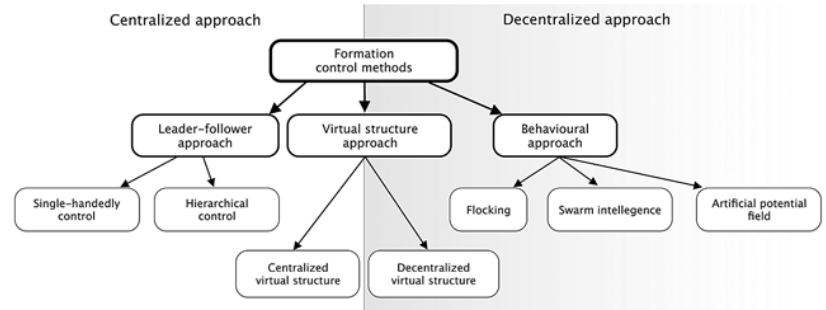
\includegraphics[width=0.62\textwidth]{figures/klasifikasi_metode_kontrol_formasi.png}}
    \hfill
    \subcaptionbox{Representasi formasi \cite{ohSurveyMultiagentFormation2015}\label{fig:klasifikasi-representasi-formasi}}[0.35\textwidth]{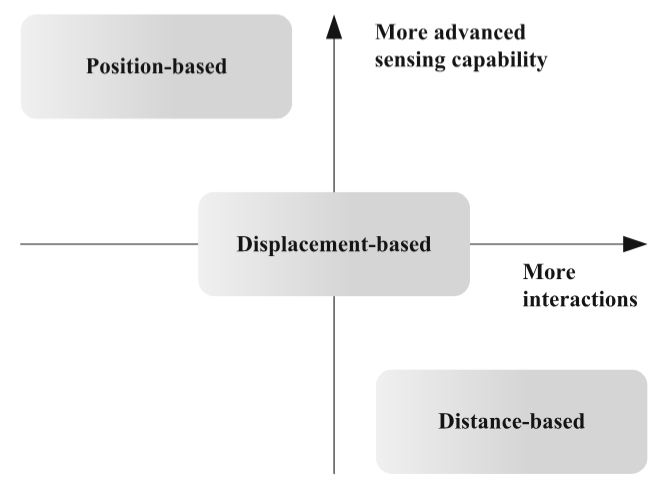
\includegraphics[width=0.35\textwidth]{figures/klasifikasi_representasi_formasi.png}}
    \caption{Klasifikasi kontrol formasi berdasarkan (a) metode dan (b) representasi.}
    \label{fig:klasifikasi_formasi}
\end{figure}

Terkait penghindaran rintangan, metode \textit{Artificial Potential Field} (APF) banyak diterapkan karena beban komputasinya yang ringan \cite{wangUAVFormationObstacle2021}. Untuk mengatasi kelemahan klasik APF berupa jebakan minimum lokal pada ruang padat, metode \textit{Improved Artificial Potential Field} (IAPF) menambahkan gaya acak dan kontrol formasi \cite{wangUAVFormationObstacle2021}. Dalam skenario ruang sempit, Bui \textit{et al.} \cite{buiEventbasedReconfigurationControl2025} mengusulkan skema \textit{Event-Based Reconfiguration Control} (ERC) yang memungkinkan formasi multi-agen beralih secara otomatis antara formasi nominal dan formasi mengekor (\textit{tailgating}) hanya saat sensor persepsi mendeteksi penyempitan batas ruang.

Pada penelitian pendahuluan terdahulu, penulis memadukan konsep ERC bersama IAPF untuk dinamika kawanan lima \textit{quadcopter} dalam simulasi komputasional 3D \cite{herdianDecentralizedFormationControl2026}. Hasil simulasi membuktikan keberhasilan rekonfigurasi adaptif terdesentralisasi saat melintasi celah sempit dengan efisiensi komunikasi tinggi. Kendati demikian, studi tersebut masih berbasis komputasi numerik murni sehingga belum memperhitungkan batasan platform fisik, seperti latensi jaringan Wi-Fi lokal, derau sensor lokalisasi kamera dan jarak, serta keterbatasan komputasi \textit{onboard}.

Implementasi fisik kontrol formasi terdesentralisasi telah didemonstrasikan oleh Quan \textit{et al.} \cite{quanDistributedSwarmTrajectory2022b, quanRobustEfficientTrajectory2023} melalui optimisasi lintasan terdistribusi untuk terbang formasi di lingkungan padat rintangan, yang menunjukkan bahwa sistem terdesentralisasi dapat bekerja andal di dunia nyata bila kendala perangkat keras ditangani sejak perancangan. Posisi penelitian tesis ini melangkah lebih jauh menjembatani celah realitas tersebut dengan merealisasikan algoritma ERC dan IAPF secara langsung pada platform perangkat keras fisik lima wahana di ruang sempit nyata. Perbandingan komparatif penelitian ini terhadap literatur kendali formasi berbasis kejadian dan ERC dirangkum pada Tabel~\ref{tab:studi-terkait-rujukan}.

\begin{table}[htbp]
    \centering
    \caption{Perbandingan komparatif penelitian tesis terhadap studi kontrol formasi berbasis kejadian (ERC)}
    \label{tab:studi-terkait-rujukan}
    \begingroup
    \footnotesize
    \setlength{\tabcolsep}{3.5pt}
    \renewcommand{\arraystretch}{1.25}
    \begin{tabularx}{\textwidth}{|>{\raggedright\arraybackslash}p{2.3cm}|>{\raggedright\arraybackslash}p{2.3cm}|>{\raggedright\arraybackslash}p{2.0cm}|>{\centering\arraybackslash}p{1.8cm}|>{\raggedright\arraybackslash}X|}
        \hline
        \rowcolor{gray!20}
        \thead{Peneliti \&\\Tahun} & \thead{Metode\\Formasi} & \thead{Skema\\Pemicu} & \thead{Platform\\\& Skala} & \thead{Karakteristik \&\\Celah Riset} \\ \hline
        Bui \textit{et al.} (2025) \cite{buiEventbasedReconfigurationControl2025} & ERC + APF & Berbasis kejadian (kondisi lingkungan) & Simulasi dan uji SIL & Pengusul ERC: peralihan antara formasi yang diinginkan dan formasi garis lurus pada lorong sempit; belum ada eksperimen fisik. \\ \hline
        Herdian \textit{et al.} (2026) \cite{herdianDecentralizedFormationControl2026} & ERC + IAPF & Berbasis kejadian terdesentralisasi & Simulasi (5 quadcopter 3D) & Formulasi integrasi ERC dan IAPF pada dinamika 3D quadcopter di lorong sempit; belum divalidasi pada platform fisik riil. \\ \hline
        \textbf{Penelitian Tesis Ini} & \textbf{ERC + IAPF} & \textbf{Berbasis kejadian terdesentralisasi} & \textbf{Fisik (5 unit SpeedyBee Bee35)} & \textbf{Validasi empiris penuh pada platform fisik lima wahana di koridor sempit; evaluasi efisiensi komunikasi MAVLink UDP, latensi nirkabel, dan kendala fisik nyata.} \\ \hline
    \end{tabularx}
    \endgroup
\end{table}

\section{Quadcopter}
Quadcopter, dengan empat motornya, merupakan sistem mekatronika dari konsep robot terbang \textit{Unmanned Aerial Vehicle} (UAV) dengan interaksi antara gaya aerodinamika, dinamika rotasi motor, dan gerakan bodi tegar secara keseluruhan untuk menentukan perilaku terbangnya. Motor diletakkan pada sudut-sudut dari quadcopter yang dapat dilihat seperti pada Gambar~\ref{fig:quadcopter-speedybee35}.

\begin{figure}[htbp]
    \centering
    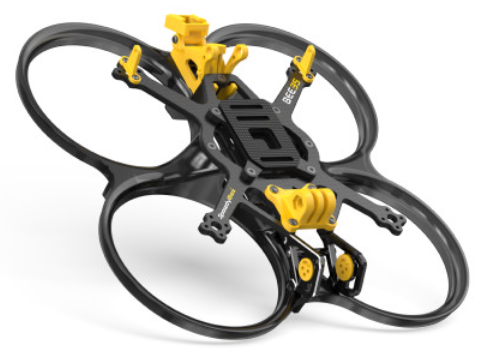
\includegraphics[width=0.5\textwidth]{figures/quadcopter_speedybee35.png}
    \caption{Quadcopter dengan kerangka SpeedyBee35 \cite{SpeedyBeeBee3535a}}
    \label{fig:quadcopter-speedybee35}
\end{figure}

Terdapat dua konfigurasi pemasangan motor yang umum digunakan pada quadcopter, yaitu konfigurasi ``+'' dan konfigurasi ``X''. Pada konfigurasi ``+'', lengan quadcopter sejajar dengan sumbu longitudinal dan lateral wahana, sehingga satu motor berada pada arah depan, satu motor pada arah belakang, dan dua motor lainnya berada pada sisi kanan serta kiri. Sementara itu, pada konfigurasi ``X'', lengan quadcopter membentuk sudut sekitar $45^{\circ}$ terhadap sumbu longitudinal dan lateral. Konfigurasi ``X'' banyak digunakan karena arah depan wahana berada di antara dua lengan, sehingga area pemasangan sensor atau kamera pada bagian depan relatif lebih terbuka. Ilustrasi perbedaan kedua konfigurasi tersebut ditunjukkan pada Gambar~\ref{fig:konfigurasi-quadcopter-plus-x}.

Pengontrolan quadcopter dicapai dengan memanipulasi kecepatan putar keempat motor. Gerakan vertikal atau perubahan ketinggian dihasilkan dengan menaikkan atau menurunkan kecepatan seluruh motor secara bersamaan sehingga resultan gaya dorong total berubah. Sebaliknya, gerakan rotasi seperti \textit{roll}, \textit{pitch}, dan \textit{yaw} diperoleh dengan memberikan perbedaan kecepatan antar motor. Perbedaan gaya dorong pada sisi kanan dan kiri menghasilkan momen \textit{roll}, perbedaan gaya dorong pada sisi depan dan belakang menghasilkan momen \textit{pitch}, sedangkan perbedaan torsi reaksi antara pasangan motor yang berputar searah dan berlawanan arah jarum jam menghasilkan momen \textit{yaw}. Dengan demikian, perubahan posisi dan orientasi quadcopter merupakan hasil kombinasi dari gaya dorong total dan momen diferensial yang diberikan oleh aktuator motor.

Dalam pemodelan dinamika quadcopter, digunakan dua kerangka acuan utama, yaitu kerangka acuan inersia dan kerangka acuan bodi. Kerangka acuan inersia $N$ dianggap tetap terhadap permukaan bumi dan digunakan sebagai referensi absolut untuk menyatakan posisi serta orientasi wahana. Konvensi yang umum digunakan adalah NED (\textit{North-East-Down}), dengan sumbu $x_N$ mengarah ke utara, sumbu $y_N$ mengarah ke timur, dan sumbu $z_N$ mengarah ke bawah. Pada konvensi ini, percepatan gravitasi bernilai positif pada arah sumbu $z_N$.

Kerangka acuan bodi $B$ melekat kaku pada quadcopter dengan titik asal umumnya ditempatkan pada pusat massa wahana. Sumbu-sumbu pada kerangka bodi dipilih mengikuti geometri utama wahana sehingga besaran seperti kecepatan linear bodi, kecepatan sudut, gaya dorong motor, dan torsi aktuator dapat dinyatakan secara lebih langsung. Dalam penelitian ini, kerangka bodi menggunakan konvensi FRD (\textit{Front-Right-Down}), yaitu sumbu $x_B$ mengarah ke depan quadcopter, sumbu $y_B$ mengarah ke kanan, dan sumbu $z_B$ mengarah ke bawah. Hubungan antara kerangka inersia NED dan kerangka bodi FRD ditunjukkan pada Gambar~\ref{fig:kerangka-acuan-ned-frd}.

\begin{figure}[htbp]
    \centering
    \subcaptionbox{Konfigurasi ``+'' dan ``X''\label{fig:konfigurasi-quadcopter-plus-x}}[0.59\textwidth]{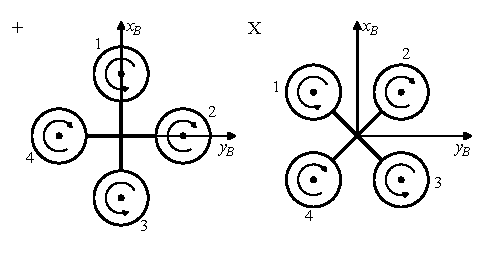
\includegraphics{figures/konfigurasi-quad.pdf}}
    \hfill
    \subcaptionbox{Kerangka NED dan FRD\label{fig:kerangka-acuan-ned-frd}}[0.39\textwidth]{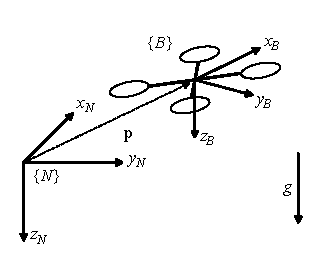
\includegraphics{figures/kerangka-ned-frd.pdf}}
    \caption[Konfigurasi motor dan kerangka acuan quadcopter.]{Konfigurasi motor dan kerangka acuan quadcopter, diadaptasi dari \cite{quanDynamicModelingExperiment2020}. (a) Tampak atas; angka menandai baling-baling, busur menandai arah putar. (b) Kerangka inersia $\{N\}$ dan kerangka bodi $\{B\}$ dengan posisi $\mathbf{p}$.}
    \label{fig:konfigurasi_kerangka}
\end{figure}

\subsection{Model Dinamika Sistem Quadcopter}
Model dinamika quadcopter pada penelitian ini dirumuskan dalam kerangka inersia NED dan kerangka bodi FRD. Penurunan persamaan gerak dilakukan menggunakan Metode Kane karena metode ini dapat menyusun dinamika benda tegar secara sistematis melalui koordinat umum, kecepatan umum, serta daftar gaya dan torsi yang bekerja pada sistem \cite{kaneDynamicsTheoryApplications1985}. Keadaan sistem dinyatakan oleh posisi pusat massa, orientasi, kecepatan translasi, dan kecepatan sudut bodi. Orientasi direpresentasikan menggunakan quaternion untuk menghindari singularitas yang umum muncul pada representasi sudut Euler. Dengan demikian, vektor keadaan plant yang digunakan ditunjukkan pada Persamaan~\ref{eq:state-plant-quadcopter}.
\begin{equation}
    \mathbf{s}_{\mathrm{plant}} =
    \begin{bmatrix}
        x & y & z & q_w & q_x & q_y & q_z & \dot{x} & \dot{y} & \dot{z} & p & q & r
    \end{bmatrix}^{T},
    \label{eq:state-plant-quadcopter}
\end{equation}
di mana $(x,y,z)$ adalah posisi pusat massa pada kerangka $N$, $(q_w,q_x,q_y,q_z)$ adalah quaternion orientasi bodi terhadap kerangka inersia, sedangkan $(p,q,r)$ adalah kecepatan sudut bodi terhadap sumbu $x_B$, $y_B$, dan $z_B$.

Kinematika translasi diperoleh dari turunan posisi pusat massa, sedangkan kinematika rotasi dinyatakan melalui hubungan antara turunan quaternion dan kecepatan sudut bodi. Hubungan kinematika quaternion tersebut diringkas pada Persamaan~\ref{eq:quaternion-kinematics}.
\begin{equation}
    \dot{\mathbf{q}} = \frac{1}{2}\mathbf{Q}(\mathbf{q})
    \begin{bmatrix}
        p & q & r
    \end{bmatrix}^{T},
    \label{eq:quaternion-kinematics}
\end{equation}
dengan $\mathbf{q}=[q_w\ q_x\ q_y\ q_z]^T$ dan $\mathbf{Q}(\mathbf{q})$ merupakan matriks transformasi quaternion. Selama simulasi, quaternion dinormalisasi agar memenuhi kendala $q_w^2+q_x^2+q_y^2+q_z^2=1$.

Dinamika translasi quadcopter ditentukan oleh gaya gravitasi, gaya dorong total motor, dan gaya hambat aerodinamis. Bentuk ringkas persamaan gaya translasi ditunjukkan pada Persamaan~\ref{eq:translational-dynamics}.
\begin{equation}
    m\ddot{\mathbf{p}} = \mathbf{F}_g + \mathbf{R}_{B}^{N}\mathbf{F}_T + \mathbf{F}_{\mathrm{drag}},
    \label{eq:translational-dynamics}
\end{equation}
Pada Persamaan~\ref{eq:translational-dynamics}, $m$ adalah massa quadcopter, $\mathbf{R}_{B}^{N}$ adalah matriks rotasi dari kerangka bodi ke kerangka inersia, dan $\mathbf{F}_T$ adalah resultan gaya dorong motor pada kerangka bodi. Untuk konvensi FRD, gaya dorong motor bekerja berlawanan arah dengan sumbu $z_B$, sehingga resultan gaya dorong total dinyatakan pada Persamaan~\ref{eq:total-thrust}.
\begin{equation}
    \mathbf{F}_T =
    \begin{bmatrix}
        0 & 0 & -(T_1+T_2+T_3+T_4)
    \end{bmatrix}^{T}.
    \label{eq:total-thrust}
\end{equation}

Dinamika rotasi diperoleh dari keseimbangan momen pada bodi quadcopter. Dengan tensor inersia $\mathbf{I}=\mathrm{diag}(I_{xx},I_{yy},I_{zz})$, bentuk ringkas persamaan rotasi ditunjukkan pada Persamaan~\ref{eq:rotational-dynamics}.
\begin{equation}
    \mathbf{I}\dot{\boldsymbol{\omega}} + \boldsymbol{\omega}\times(\mathbf{I}\boldsymbol{\omega})
    = \boldsymbol{\tau}_{T} + \boldsymbol{\tau}_{M} + \boldsymbol{\tau}_{\mathrm{gyro}},
    \label{eq:rotational-dynamics}
\end{equation}
Pada Persamaan~\ref{eq:rotational-dynamics}, $\boldsymbol{\omega}=[p\ q\ r]^T$, $\boldsymbol{\tau}_{T}$ adalah momen akibat perbedaan gaya dorong antar motor, $\boldsymbol{\tau}_{M}$ adalah torsi reaktif motor, dan $\boldsymbol{\tau}_{\mathrm{gyro}}$ adalah torsi giroskopik rotor. Untuk konfigurasi ``X'', kombinasi perbedaan gaya dorong motor menghasilkan momen \textit{roll} dan \textit{pitch}, sedangkan perbedaan torsi reaktif pasangan motor menghasilkan momen \textit{yaw}.

Gaya dorong dan torsi reaktif masing-masing motor dimodelkan sebagai fungsi kuadrat dari kecepatan sudut motor, seperti ditunjukkan pada Persamaan~\ref{eq:motor-thrust-torque}.
\begin{equation}
    T_i = k_T\omega_i^2, \qquad \tau_i = k_Q\omega_i^2,
    \label{eq:motor-thrust-torque}
\end{equation}
dengan $k_T$ sebagai koefisien gaya dorong dan $k_Q$ sebagai koefisien torsi. 

Respons aktuator motor pada wahana fisik dikendalikan secara langsung oleh unit ESC 4-in-1 melalui sinyal komando digital berfrekuensi tinggi, sehingga dinamika putaran motor memiliki konstanta waktu yang jauh lebih cepat dibandingkan dinamika translasi bodi quadcopter. 

Untuk keperluan simulasi numerik komputasional dan pengujian \textit{Hardware-In-The-Loop} (HITL) pada tahap awal penelitian, dinamika bodi 13-\textit{state} (Persamaan~\ref{eq:state-plant-quadcopter}) digabungkan dengan pemodelan transien aktuator motor orde kedua membentuk model non-linear 21-\textit{state} \cite{johnBobzwikQuadcopter_SimCon2025, kaneDynamicsTheoryApplications1985}. Sementara itu, pada implementasi fisik di lingkungan dalam ruangan, tugas stabilisasi sikap dan regulasi gaya dorong motor didelegasikan sepenuhnya kepada kalang kontrol PID kaskade pada \textit{Flight Controller} (FC), sebagaimana dirinci pada Bab~\ref{sec:arsitektur_sistem}. Dengan demikian, model translasi bodi kaku pada Persamaan~\ref{eq:translational-dynamics} dan model orientasi pada Persamaan~\ref{eq:quaternion-kinematics} menjadi acuan utama bagi perencana tingkat tinggi di \textit{companion computer} dalam menghasilkan referensi trajektori formasi kawanan.


% ==========================================
% BAB III PERANCANGAN SISTEM
% ==========================================
\chapter{PERANCANGAN SISTEM}

Bab ini memuat keputusan perancangan: perangkat yang dipilih, parameter yang ditetapkan, geometri wahana, dan arena uji. Uraian dimulai dari kondisi awal perangkat, dilanjutkan rancangan tiap subsistem, dan ditutup arsitektur sistem menyeluruh.

\section{Kondisi Awal dan Komponen yang Tersedia}
\label{sec:kondisi_awal}

Sebagian perangkat keras telah tersedia di laboratorium sebagai kelanjutan platform penelitian sebelumnya \cite{argilianaPengembanganSistemKontrol2025}. Perancangan hanya melengkapi bagian yang belum ada, dan pemetaan ini menjadi dasar anggaran pada Bab~IV.

\subsection{Wahana dan Komponen Elektronik}

Wahana yang digunakan adalah \textit{quadcopter} tipe \textit{cinewhoop} dengan propeler bersaluran, berdimensi luar $25 \times 21$ cm dan tinggi $8$ cm termasuk baterai. Bentuk bersaluran menutupi propeler secara penuh sehingga lebih aman untuk penerbangan berdekatan dengan dinding dan rintangan. Rincian komponen yang telah tersedia dirangkum pada Tabel~\ref{tab:komponen_tersedia}.

\begin{table}[htbp]
    \centering
    \caption{Komponen yang telah tersedia di laboratorium}
    \label{tab:komponen_tersedia}
    \begingroup
    \small
    \setlength{\tabcolsep}{4pt}
    \renewcommand{\arraystretch}{1.3}
    \begin{tabularx}{\textwidth}{|c|>{\raggedright\arraybackslash}p{3.6cm}|>{\raggedright\arraybackslash}X|>{\centering\arraybackslash}p{1.6cm}|}
        \hline
        \rowcolor{gray!20}
        \thead{No} & \thead{Komponen} & \thead{Spesifikasi} & \thead{Jumlah} \\ \hline
        1 & Rangka \textit{cinewhoop} SpeedyBee Bee35 & Propeler bersaluran, dimensi luar $25 \times 21 \times 8$ cm & 6 unit \\ \hline
        2 & Motor BLDC & $2006$, $1950$ KV & 4 per wahana \\ \hline
        3 & \textit{Flight controller} SpeedyBee F405 Mini & Mikrokontroler STM32F405 (\textit{flash} 1 MB), IMU ICM-42688P, barometer DSP-310 & 4 unit \\ \hline
        4 & ESC SpeedyBee BLS 35A Mini & 4-in-1, firmware BLHeli\_S & 4 unit \\ \hline
        5 & \textit{Companion computer} Seeed XIAO ESP32-S3 & Wi-Fi 2,4 GHz dan BLE terintegrasi, antarmuka USB-C & 1 unit \\ \hline
        6 & Penerima kendali radio ExpressLRS EP2 TCXO & 2,4 GHz; pemancar belum tersedia & 3 unit \\ \hline
        7 & Baterai LiPo & $4 \times 1200$ mAh, $2 \times 1500$ mAh, $1 \times 2200$ mAh, $2 \times 5000$ mAh & 9 unit \\ \hline
        8 & Propeler dan saluran cadangan & Propeler tiga bilah, cincin saluran & beberapa \\ \hline
        9 & Modul navigasi RUSHFPV GNSS 25+ & Mesin u-Blox M10, kompas HMC5883, antarmuka serial 115200 baud & terpasang \\ \hline
        10 & Pencetak tiga dimensi beserta filamen & Untuk mencetak dudukan penanda visual dan sensor & 1 unit \\ \hline
        11 & Pengisi daya baterai, komputer stasiun darat, dan penghala Wi-Fi khusus & Perangkat pendukung di sisi darat & tersedia \\ \hline
    \end{tabularx}
    \endgroup
\end{table}

Dari enam rangka yang tersedia, dua unit telah terpasang lengkap beserta propeler dan siap diterbangkan, dua unit telah terpasang motor dan saluran namun belum berpropeler, sementara dua unit sisanya masih berupa rangka kosong tanpa komponen elektronik. Dengan demikian kebutuhan lima agen dapat dipenuhi dari stok yang ada, dengan satu unit tersisa sebagai cadangan apabila terjadi kerusakan saat uji terbang.

Modul navigasi RUSHFPV yang terpasang pada bagian atas wahana memuat penerima GNSS sekaligus magnetometer HMC5883. Penerima GNSS tidak dapat digunakan karena seluruh pengujian berlangsung di dalam ruangan. Magnetometer secara prinsip masih dapat menjadi acuan arah, namun pembacaannya di dalam gedung mudah terganggu struktur baja dan kabel daya, sehingga acuan \textit{yaw} diambil dari sistem kamera atas. Dengan demikian modul tersebut dilepas, dan pelepasannya justru menguntungkan: bobot berkurang, dan area datar di tengah bodi yang dibutuhkan untuk pemasangan penanda visual menjadi bebas, sebagaimana dibahas pada Subbab~\ref{sec:lokalisasi_rancangan}.

\subsection{Kondisi Ruang Pengujian}
\label{subsec:kondisi_ruang}

Pengujian eksperimental dilaksanakan di koridor Pusat Teknologi Instrumentasi dan Otomasi (PTIO) ITB. Ruangan tersebut bukan laboratorium terbang khusus, melainkan koridor berbentuk huruf L yang juga digunakan sebagai area lalu lintas dan kegiatan pelatihan. Karakteristik ruang yang relevan terhadap perancangan dirangkum pada Tabel~\ref{tab:kondisi_ruang}.

\begin{table}[htbp]
    \centering
    \caption{Karakteristik ruang pengujian yang relevan terhadap perancangan}
    \label{tab:kondisi_ruang}
    \begingroup
    \small
    \setlength{\tabcolsep}{4pt}
    \renewcommand{\arraystretch}{1.3}
    \begin{tabularx}{\textwidth}{|>{\raggedright\arraybackslash}p{4.0cm}|>{\raggedright\arraybackslash}p{3.0cm}|X|}
        \hline
        \rowcolor{gray!20}
        \thead{Karakteristik} & \thead{Nilai} & \thead{Konsekuensi terhadap perancangan} \\ \hline
        Tinggi langit-langit & $300$ cm & Membatasi jarak pandang kamera atas terhadap wahana, sehingga liputan satu kamera terbatas \\ \hline
        Lebar bersih lengan koridor & $270$ cm & Membatasi bentang formasi maksimum yang dapat diuji \\ \hline
        Panjang lengan koridor & $720$--$960$ cm & Menentukan panjang lintasan uji yang tersedia \\ \hline
        Jenis langit-langit & Gipsum pada rangka-T, ubin $60 \times 60$ cm & Dudukan kamera harus ringan dan mencantol pada rel rangka; posisi ubin yang terpakai pendingin, lampu, dan \textit{sprinkler} harus dihindari \\ \hline
        Pencahayaan & Lampu TL, lampu tanam, dan kaca \textit{clerestory} & Suhu warna dan intensitas tidak seragam; pengaturan pencahayaan otomatis kamera harus dikunci manual \\ \hline
        Lantai & Ubin besar berwarna gelap & Kontras baik terhadap penanda visual berwarna terang; nat ubin dapat dipakai menandai posisi rintangan secara berulang \\ \hline
        Kolom di dalam area & $4$ buah, $45$--$60$ cm & Salah satu kolom dimanfaatkan sebagai sisi penyempitan pada arena uji \\ \hline
        Status penggunaan & Dapat dipakai eksklusif dengan penjadwalan & Perabot dapat disingkirkan saat sesi pengujian sehingga lebar bersih penuh tersedia \\ \hline
    \end{tabularx}
    \endgroup
\end{table}

Seluruh ukuran pada Tabel~\ref{tab:kondisi_ruang} diperoleh melalui pengukuran langsung di lokasi dengan ketelitian sekitar $\pm 5$ cm. Pada kondisi sehari-hari, sebagian lebar koridor terpakai oleh deretan kursi panjang, papan informasi berdiri, dan perlengkapan laboratorium. Karena ruangan dapat dijadwalkan untuk penggunaan eksklusif, perabot tersebut disingkirkan selama sesi pengujian sehingga lebar bersih $270$ cm dapat dimanfaatkan sepenuhnya. Ketersediaan lebar penuh ini merupakan syarat yang mengikat: dengan perabot tetap di tempatnya, lebar bersih hanya sekitar $180$ cm dan bentang formasi yang dirancang tidak akan muat, sehingga peristiwa pemicu rekonfigurasi tidak akan terjadi secara sah.

\section{Arsitektur Wahana}
Wahana eksperimental adalah quadcopter konfigurasi X berbasis rangka SpeedyBee Bee35 (Gambar~\ref{fig:quadcopter-speedybee35}), kelanjutan platform penelitian sebelumnya \cite{argilianaPengembanganSistemKontrol2025}. Komponen dibagi dua lapis: \textit{companion computer} di sisi atas, sedangkan \textit{flight controller} (FC\label{abbr:fc}) dan \textit{Electronic Speed Controller} (ESC\label{abbr:esc}) di inti kerangka (Gambar~\ref{fig:struktur_fisik}).

\begin{figure}[htbp]
    \centering
    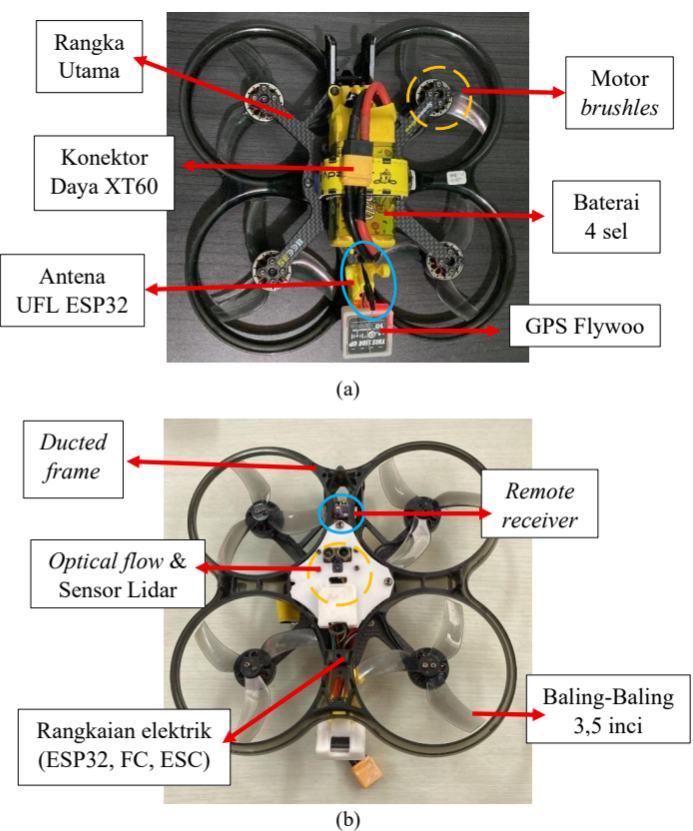
\includegraphics[width=0.55\textwidth]{figures/struktur_fisik.png}
    \caption{Struktur fisik dan tata letak komponen: (a) tampak atas dan (b) tampak bawah \cite{argilianaPengembanganSistemKontrol2025}}
    \label{fig:struktur_fisik}
\end{figure}

FC dan ESC 4-in-1 tersusun sebagai satu tumpukan vertikal. FC memuat IMU dan mengirim komando motor ke ESC, yang menggerakkan keempat motor BLDC. Tumpukan dipasang di atas peredam getaran silikon untuk mengurangi derau getaran motor pada IMU (Gambar~\ref{fig:esc_fc}).

\begin{figure}[htbp]
    \centering
    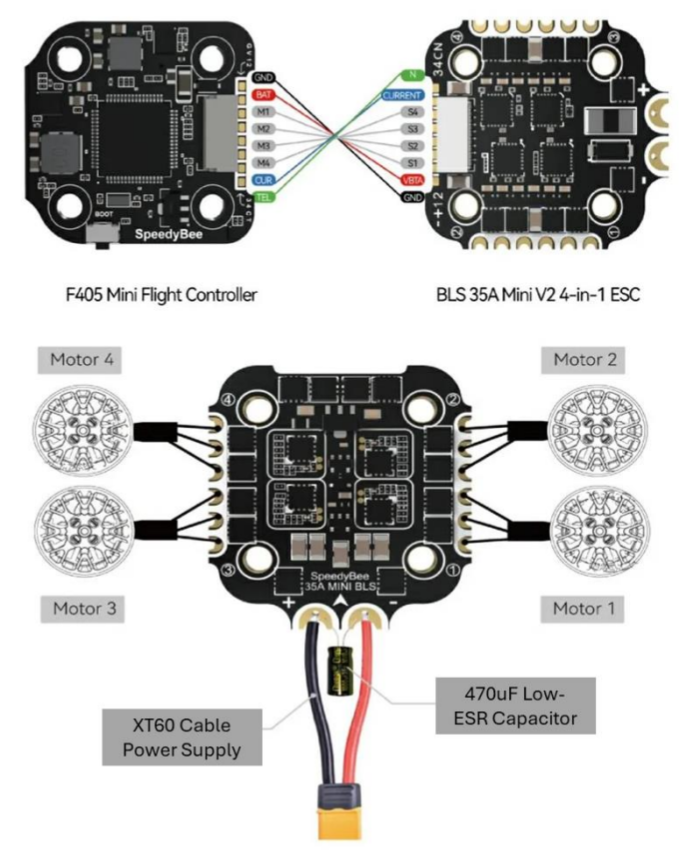
\includegraphics[width=0.45\textwidth]{figures/esc_fc.png}
    \caption{Tumpukan \textit{flight controller} dan ESC 4-in-1}
    \label{fig:esc_fc}
\end{figure}

Baterai LiPo mencatu ESC, yang menyalurkan daya teregulasi ke FC melalui BEC (\textit{Battery Eliminator Circuit}). XIAO ESP32-S3 terhubung ke FC melalui UART dengan TX dan RX disilangkan untuk pertukaran MAVLink, dan penerima ExpressLRS EP2 TCXO terhubung ke FC untuk kendali manual (Gambar~\ref{fig:wiring_diagram}). Modul GNSS pada gambar tersebut dilepas pada penelitian ini (Subbab~\ref{sec:kondisi_awal}).

\begin{figure}[htbp]
    \centering
    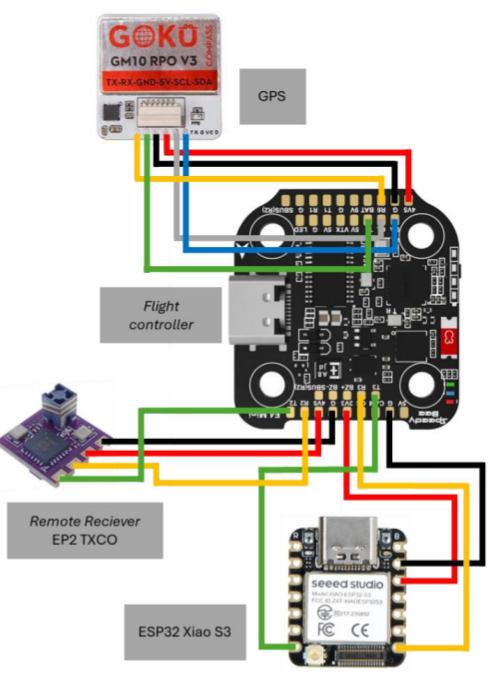
\includegraphics[width=0.35\textwidth]{figures/wiring_diagram.png}
    \caption{Diagram pengabelan wahana}
    \label{fig:wiring_diagram}
\end{figure}

\subsection{Dimensi dan Tata Letak Komponen}

Tata letak dan dimensi luar wahana diperlihatkan pada Gambar~\ref{fig:sketsa_wahana}. Empat saluran propeler menempati hampir seluruh permukaan atas, menyisakan jalur datar selebar hanya $4$ cm di sepanjang sumbu tengah bodi. Keterbatasan ruang datar ini berdampak langsung pada perancangan sistem lokalisasi dan dibahas pada Subbab~\ref{sec:lokalisasi_rancangan}.

\begin{figure}[htbp]
    \centering
    \subcaptionbox{Tampak atas wahana (cm)\label{fig:sketsa_wahana}}[0.49\textwidth]{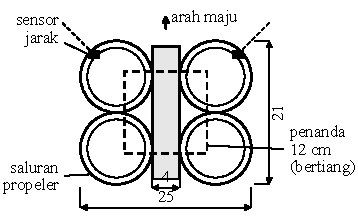
\includegraphics{figures/wahana-atas.pdf}}
    \hfill
    \subcaptionbox{Geometri estimasi lebar ruang\label{fig:ultrasonic_placement}}[0.49\textwidth]{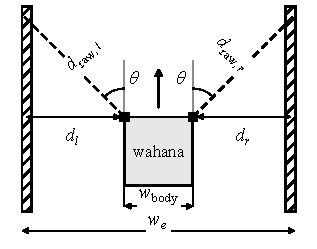
\includegraphics{figures/geometri-we.pdf}}
    \caption{Wahana uji dan penempatan sensor jarak. (a) Empat saluran propeler menyisakan jalur datar selebar $4$~cm di sumbu tengah; penanda $12$~cm dipasang bertiang di atasnya. (b) Dua sensor diagonal bersudut $\beta$ terhadap arah maju menghasilkan jarak lateral $d_l$ dan $d_r$ untuk estimasi $w_e$.}
    \label{fig:wahana_sensor}
\end{figure}

\subsection{Protokol Komunikasi}
Seluruh komunikasi data memakai pesan MAVLink di atas soket UDP pada jaringan Wi-Fi lokal \cite{chenReviewUnmannedAerial2020, linLeaderFollowerUAV2026}. Jaringan dibentuk oleh satu \textit{router} khusus di area uji dan memuat dua jalur:
\begin{enumerate}
    \item \textbf{Antarwahana.} Tiap ESP32-S3 menyiarkan \textit{state} kinematikanya (posisi dan kecepatan) melalui UDP \textit{broadcast}. \textit{Router} hanya meneruskan paket; keputusan rekonfigurasi tetap diambil oleh tiap agen.
    \item \textbf{Stasiun darat.} Stasiun darat menyiarkan pose hasil kamera atas dan menerima telemetri (\textit{heartbeat}, sikap, dan tegangan baterai), serta mengirim perintah \textit{arm/disarm}, pergantian mode, dan pendaratan darurat.
\end{enumerate}
Karena kedua jalur melewati \textit{router} yang sama, kegagalan \textit{router} memutus pose dan komunikasi antaragen sekaligus. Jalur penghentian yang tidak bergantung pada Wi-Fi karenanya disediakan melalui tautan radio ExpressLRS (Gambar~\ref{fig:arsitektur_sistem}).

\section{Perancangan Sistem Lokalisasi Dalam Ruangan}
\label{sec:lokalisasi_rancangan}

GPS tidak tersedia di dalam ruangan, sehingga posisi absolut diperoleh dari kamera atas yang mengamati penanda visual pada wahana. Lokalisasi kamera eksternal tidak mengakumulasi \textit{drift}: galat pose di bawah $3$~cm dan $1^\circ$ telah dilaporkan untuk area dalam ruangan seluas sekitar $240$~m$^2$ \cite{bultmannExternalCameraBased2023}. Presisinya bergantung pada resolusi kamera, ukuran penanda, dan jarak kamera ke penanda; akurasi pose AprilTag menurun seiring bertambahnya jarak dan mengecilnya penanda \cite{zhangIntegratedFrameworkEnhancing2026}. Ketiga besaran tersebut karenanya dihitung dari dimensi ruang uji (Subbab~\ref{subsec:liputan_kamera}).

Sistem lokalisasi terdiri atas tiga komponen:
\begin{enumerate}
    \item \textbf{Kamera atas.} Dua kamera dipasang statis di langit-langit menghadap tegak lurus ke bawah. Liputannya bertumpang tindih dan dikalibrasi ke satu kerangka acuan global, karena tinggi langit-langit membatasi liputan satu kamera.
    \item \textbf{Penanda visual.} Tiap wahana membawa penanda AprilTag \cite{olsonAprilTagRobustFlexible2011, wangAprilTag2Efficient2016, krogiusFlexibleLayoutsFiducial2019}, keluarga penanda biner sejenis ArUco \cite{garridojuradoAutomaticGenerationDetection2014}, dengan ID unik (0 hingga 4) sehingga kelima agen dapat dibedakan.
    \item \textbf{Stasiun pemroses citra.} Komputer darat menerima aliran video, mendeteksi penanda, dan menghitung pose tiap wahana.
\end{enumerate}

Pose tiap wahana dihitung dengan model kamera lubang jarum dan penyelesaian masalah \textit{Perspective-n-Point} (PnP). Dengan matriks intrinsik $\mathbf{K}$ yang diperoleh dari kalibrasi, koordinat piksel $(u, v)$ dan koordinat dunia $(x_w, y_w, z_w)$ berhubungan melalui
\begin{equation}
    s 
    \begin{bmatrix}
        u \\ v \\ 1
    \end{bmatrix}
    = \mathbf{K} 
    \begin{bmatrix}
        \mathbf{R} & \mathbf{T}
    \end{bmatrix}
    \begin{bmatrix}
        x_w \\ y_w \\ z_w \\ 1
    \end{bmatrix}
    \label{eq:pinhole_pnp}
\end{equation}
dengan $s$ faktor skala, $\mathbf{R} \in \mathbb{R}^{3 \times 3}$ matriks rotasi, $\mathbf{T} \in \mathbb{R}^3$ vektor translasi, dan
\begin{equation}
    \mathbf{K} = 
    \begin{bmatrix}
        f_x & 0 & c_x \\
        0 & f_y & c_y \\
        0 & 0 & 1
    \end{bmatrix}
\end{equation}
dengan $(f_x, f_y)$ panjang fokus dalam piksel dan $(c_x, c_y)$ titik pusat optik. Dari ukuran penanda yang diketahui ($12 \times 12$~cm) dan empat titik sudutnya pada citra, Persamaan~\ref{eq:pinhole_pnp} diselesaikan secara numerik dengan optimasi Levenberg\allowbreak--Marquardt, menghasilkan posisi $(x, y, z)$ dan sudut \textit{yaw} $\psi$ tiap wahana.

Pose tersebut dikemas sebagai pesan MAVLink dan disiarkan melalui UDP ke \textit{companion computer} tiap wahana. Laju pembaruannya dibatasi laju bingkai kamera ($50$ bingkai per detik) dan tertunda oleh pemrosesan citra, sehingga pose kamera tidak diumpankan langsung ke kalang kendali, melainkan difusikan dengan IMU melalui \textit{Extended Kalman Filter} (EKF\label{abbr:ekf}).

\subsection{Penentuan Jumlah Kamera dan Ukuran Penanda}
\label{subsec:liputan_kamera}

Kamera yang dipilih adalah kamera USB \textit{global shutter} beresolusi $2592 \times 1944$ piksel (format $4{:}3$) dengan lensa $120^\circ$. Rana global dipilih karena rana bergulir memelintir citra penanda saat wahana bergerak. Liputan dan ukuran penanda diturunkan dari dimensi ruang pada Tabel~\ref{tab:kondisi_ruang}. Dengan langit-langit setinggi $h_p = 3{,}00$~m, tinggi wahana $0{,}08$~m, dan ketinggian terbang $h_t = 1{,}2$~m, jarak kamera ke penanda adalah
\begin{equation}
    d = h_p - (h_t + 0{,}08) = 1{,}72\ \text{m}
\end{equation}
Untuk sudut pandang horizontal $\gamma_h$ dan vertikal $\gamma_v$, liputan satu kamera pada bidang terbang adalah
\begin{equation}
    w_\parallel = 2d\tan\frac{\gamma_h}{2}, \qquad w_\perp = 2d\tan\frac{\gamma_v}{2}
\end{equation}
dengan $w_\parallel$ searah koridor dan $w_\perp$ melintang koridor. Lembar data kamera belum menyatakan apakah $120^\circ$ merupakan sudut horizontal atau diagonal, sehingga keduanya dihitung (Tabel~\ref{tab:liputan_kamera}).

\begin{table}[htbp]
    \centering
    \caption{Liputan satu kamera dan ukuran penanda pada ketinggian terbang $1{,}2$~m}
    \label{tab:liputan_kamera}
    \begingroup
    \small
    \renewcommand{\arraystretch}{1.25}
    \begin{tabularx}{\textwidth}{|X|>{\centering\arraybackslash}p{3.0cm}|>{\centering\arraybackslash}p{3.0cm}|}
        \hline
        \rowcolor{gray!20}
        \thead{Besaran} & \thead{$120^\circ$ horizontal} & \thead{$120^\circ$ diagonal} \\ \hline
        Liputan $w_\parallel \times w_\perp$ & $5{,}96 \times 4{,}47$ m & $4{,}77 \times 3{,}57$ m \\ \hline
        Resolusi pada bidang terbang & $2{,}30$ mm/piksel & $1{,}84$ mm/piksel \\ \hline
        Penanda $10$ cm & $44$ piksel & $54$ piksel \\ \hline
        Penanda $12$ cm & $52$ piksel & $65$ piksel \\ \hline
        Tumpang tindih dua kamera pada segmen $7{,}20$ m & $4{,}72$ m & $2{,}33$ m \\ \hline
    \end{tabularx}
    \endgroup
\end{table}

Pada kedua tafsiran, liputan melintang melebihi lebar koridor $2{,}70$~m, dan satu kamera tidak mencukupi segmen uji sepanjang $7{,}20$~m. Dua kamera menutup segmen tersebut dengan tumpang tindih sekurang-kurangnya $2{,}33$~m, yang dipakai untuk menyatukan keduanya ke satu kerangka acuan global.

Ukuran penanda ditetapkan dari syarat deteksi. Penanda dianggap terdeteksi andal bila sisinya mencakup sekurang-kurangnya $48$ piksel. Penanda $10$~cm tidak memenuhi syarat ini pada tafsiran horizontal ($44$ piksel), sedangkan penanda $12$~cm memenuhi pada kedua tafsiran. Karena itu ukuran penanda ditetapkan $12$~cm; bila lembar data menyatakan sudut diagonal, penanda $10$~cm sudah memadai. Marginnya tetap tipis terhadap $80$ piksel yang nyaman untuk wahana bergerak, sehingga keandalan deteksi saat terbang dipastikan pada uji terbang tunggal sebelum komponen kawanan dibeli (Bab~IV).

Penanda $12$~cm tidak muat pada jalur datar selebar $4$~cm di sumbu tengah bodi (Gambar~\ref{fig:sketsa_wahana}), dan menempelkannya langsung di atas saluran propeler akan menutup aliran udara masuk dan menggerus daya angkat. Penanda karenanya dipasang pada pelat yang dinaikkan tiang penyangga setinggi $7$~cm di atas bodi, dengan dudukan dicetak menggunakan pencetak tiga dimensi yang tersedia.

\section{Perancangan Sistem Persepsi Rintangan}

Pemicu ERC membutuhkan lebar ruang bebas yang diukur sendiri oleh tiap agen. Untuk itu setiap wahana membawa sepasang sensor jarak yang dipasang diagonal, satu di kiri dan satu di kanan, bersudut $\beta$ terhadap arah maju (Gambar~\ref{fig:ultrasonic_placement}). Jenis sensornya, ultrasonik atau laser, ditetapkan melalui uji banding pada Subbab~\ref{subsec:pemilihan_sensor}.

Kandidat ultrasonik mengukur jarak dari waktu tempuh pantulan gelombang suara \cite{siegwartIntroductionAutonomousMobile2004, borensteinObstacleAvoidanceUltrasonic1988}:
\begin{equation}
    d_{\text{obs}} = \frac{v_{\text{suara}} \cdot t_{\text{pantul}}}{2}
\end{equation}
dengan $v_{\text{suara}}$ kecepatan rambat suara di udara (sekitar $343$ m/s pada $20^\circ\text{C}$) dan $t_{\text{pantul}}$ waktu tempuh bolak-balik gelombang.

Jarak terukur sepanjang berkas, $d_{\mathrm{raw}}$, diproyeksikan menjadi jarak lateral kiri ($d_l$\label{sym:dl}) dan kanan ($d_r$\label{sym:dr}) oleh \textit{companion computer}:
\begin{equation}
    d_l = d_{\mathrm{raw},l}\sin\beta, \qquad d_r = d_{\mathrm{raw},r}\sin\beta
\end{equation}
Lebar ruang bebas ($w_e$\label{sym:we}) tegak lurus arah gerak adalah
\begin{equation}
    w_e = d_l + d_r + w_{\text{body}}
\end{equation}
dengan $w_{\text{body}}$\label{sym:wbody} jarak antarsensor pada badan wahana. Nilai $w_e$ diumpankan ke perencana tingkat tinggi dan memicu mode mengekor ketika $w_e \le \alpha R$ (Persamaan~\ref{eq:erc_pemicu}).

\subsection{Pemilihan Sensor Jarak}
\label{subsec:pemilihan_sensor}

Rancangan di atas mengandalkan pembacaan jarak lateral yang tetap andal ketika berkas sensor mengenai permukaan secara miring. Pada sudut datang $45^\circ$ terhadap permukaan halus seperti dinding berplester atau kolom beton, sensor ultrasonik rawan kehilangan gema karena pantulan bersifat spekular dan energi pantul terlempar menjauh dari penerima. Permukaan kardus yang dipakai sebagai rintangan buatan memantul secara baur sehingga lebih ramah, tetapi dinding dan kolom tidak.

Risiko ini menyentuh inti mekanisme ERC: kegagalan pembacaan pada sudut miring berarti estimasi $w_e$ menjadi tidak sahih, dan peristiwa pemicu dapat terlewat atau terpicu palsu. Oleh sebab itu jenis sensor tidak ditetapkan di muka, melainkan diputuskan melalui uji banding pada Fase~2. Dua kandidat diuji berdampingan:

\begin{enumerate}
    \item \textbf{Sensor ultrasonik} (HC-SR04). Berbiaya rendah, jangkauan memadai, dan tidak terpengaruh kondisi pencahayaan, namun memiliki resolusi sudut yang buruk akibat berkas yang lebar dan rentan terhadap pantulan spekular pada sudut datang miring \cite{pedroSenseAvoidSystem2025}.
    \item \textbf{Sensor jarak laser \textit{time-of-flight}} (VL53L1X). Berkas jauh lebih sempit, lebih toleran terhadap sudut datang miring, dan berkomunikasi melalui antarmuka I\textsuperscript{2}C sehingga hemat pena masukan-keluaran pada \textit{companion computer} yang terbatas. Sensor berbasis laser memberikan resolusi spasial yang lebih tinggi karena memakai gelombang berpanjang gelombang jauh lebih pendek \cite{pedroSenseAvoidSystem2025}. Kelemahannya, jangkauan efektifnya menurun pada pencahayaan terang, sedangkan ruang pengujian menerima cahaya alami melalui kaca \textit{clerestory}.
\end{enumerate}

Kriteria pemilihan ditetapkan sebelum pengujian dijalankan, yaitu: tingkat keberhasilan pembacaan pada sudut $45^\circ$ dan $90^\circ$ terhadap dinding berplester, kolom beton, dan permukaan kardus; sebaran galat pembacaan terhadap jarak acuan; serta laju pembaruan yang dapat dicapai untuk dua sensor sekaligus. Sensor yang memenuhi kriteria dengan margin terbesar dipakai untuk kelima wahana. Apabila kedua kandidat gagal pada sudut $45^\circ$, sudut pemasangan diperkecil dan konsekuensinya terhadap jangkauan deteksi ke depan dievaluasi ulang.

\section{Estimator dan Pengontrol}

Bagian ini menguraikan rancangan kalang estimasi dan kendali yang dijalankan di atas wahana, mulai dari fusi sensor hingga alokasi perintah motor.

\subsection{Firmware \textit{Flight Controller}}
\label{subsec:firmware_fc}

Pose dari kamera atas hanya berguna bila \textit{flight controller} dapat menerimanya sebagai sumber navigasi eksternal. ArduPilot mendukung masukan ini melalui EKF3, tetapi fitur navigasi non-GPS memerlukan papan dengan memori \textit{flash} lebih dari 1~MB \cite{ardupilotNonGPSPositionEstimation}. SpeedyBee F405 Mini hanya memiliki 1~MB, dan build stabil resminya menonaktifkan fitur navigasi eksternal EKF3, odometri visual, serta masukan \textit{beacon} \cite{ardupilotFeaturesSpeedyBeeF405Mini}. Dengan firmware bawaan, pose kamera tidak dapat diterima.

Penelitian ini karenanya memakai firmware ArduPilot racikan yang dibangun melalui ArduPilot Custom Firmware Builder \cite{ardupilotCustomFirmwareBuilder}: fitur navigasi eksternal EKF3 diaktifkan dan fitur yang tidak dipakai dinonaktifkan agar muat dalam 1~MB. Build ini dikerjakan pada Fase~2. Bila tidak muat, kalang posisi dan kecepatan dipindahkan ke \textit{companion computer}, dan \textit{flight controller} hanya menjalankan kalang sikap. Daftar fitur yang diaktifkan dan dinonaktifkan dicatat sebagai lampiran agar firmware dapat dibangun ulang.

\subsection{Estimator \textit{State} dengan \textit{Extended Kalman Filter} (EKF)}

Dinamika quadcopter tidak linear dan setiap sensor mengandung derau, sehingga \textit{state} wahana diestimasi dengan EKF \cite{KalmanFilterGeneralizations2006}. EKF memadukan IMU yang cepat tetapi mengakumulasi \textit{drift} dengan pose kamera atas yang absolut tetapi lebih lambat. Pendekatan penapis Kalman tetap lazim untuk estimasi pose wahana udara mikro di dalam ruangan dan masih dibandingkan dengan pendekatan berbasis graf pada penelitian mutakhir \cite{kabiriGraphBasedErrorState2024}.

Secara matematis, sistem estimasi \textit{state} quadcopter dirumuskan dalam model ruang keadaan non-linear diskrit \cite{welchIntroductionKalmanFilter2006}:
\begin{align}
    \mathbf{x}_k &= f(\mathbf{x}_{k-1}, \mathbf{u}_{k-1}) + \mathbf{w}_{k-1} \label{eq:ekf_system} \\
    \mathbf{z}_k &= h(\mathbf{x}_k) + \mathbf{v}_k \label{eq:ekf_measurement}
\end{align}
Formulasi berikut adalah model konseptual; implementasinya memakai EKF3 bawaan ArduPilot pada firmware racikan (Subbab~\ref{subsec:firmware_fc}), yang \textit{state}-nya lebih lengkap. Pada model konseptual ini, vektor \textit{state} $\mathbf{x}_k \in \mathbb{R}^{10}$ mencakup posisi 3D pada kerangka inersia global, kecepatan linear, dan \textit{quaternion} orientasi bodi:
\begin{equation}
    \mathbf{x} = 
    \begin{bmatrix}
        x & y & z & \dot{x} & \dot{y} & \dot{z} & q_w & q_x & q_y & q_z
    \end{bmatrix}^T
    \label{eq:state_vector_ekf}
\end{equation}
Vektor masukan $\mathbf{u}_{k-1}$ berasal dari pembacaan sensor internal IMU bawaan \textit{flight controller} (ICM-42688P) pada laju yang jauh lebih tinggi daripada laju kamera, yang terdiri atas akselerasi linear bodi $\mathbf{a}_B = [a_x, a_y, a_z]^T$ dan laju rotasi bodi $\boldsymbol{\omega}_B = [p, q, r]^T$. Sementara itu, vektor pengukuran $\mathbf{z}_k \in \mathbb{R}^4$ diperoleh secara asinkron dari sistem kamera atas berbasis penanda visual AprilTag hingga $50$ kali per detik melalui paket MAVLink:
\begin{equation}
    \mathbf{z}_k = 
    \begin{bmatrix}
        x_{\mathrm{cam}} & y_{\mathrm{cam}} & z_{\mathrm{cam}} & \psi_{\mathrm{cam}}
    \end{bmatrix}^T
    \label{eq:measurement_vector_ekf}
\end{equation}
Derau proses $\mathbf{w}_{k-1}$ dan derau pengukuran $\mathbf{v}_k$ dimodelkan sebagai derau Gaussian putih dengan kovariansi $\mathbf{Q}_k$ dan $\mathbf{R}_k$.

Karena fungsi kinematika translasi dan rotasi bersifat non-linear, EKF melakukan linearisasi lokal pada setiap langkah waktu menggunakan matriks Jacobian \cite{gelbAppliedOptimalEstimation1974}:
\begin{equation}
    \mathbf{F}_{k-1} = \left. \frac{\partial f}{\partial \mathbf{x}} \right|_{\hat{\mathbf{x}}_{k-1|k-1}, \mathbf{u}_{k-1}}, \quad \mathbf{H}_k = \left. \frac{\partial h}{\partial \mathbf{x}} \right|_{\hat{\mathbf{x}}_{k|k-1}}
\end{equation}

Proses estimasi EKF berjalan dalam arsitektur \textit{multi-rate} melalui dua tahapan utama:

\subsubsection{1. Tahap Prediksi}
Dijalankan setiap cuplikan IMU. Model kinematika memproyeksikan posisi, kecepatan, dan orientasi maju:
\begin{align}
    \hat{\mathbf{x}}_{k|k-1} &= f(\hat{\mathbf{x}}_{k-1|k-1}, \mathbf{u}_{k-1}) \\
    \mathbf{P}_{k|k-1} &= \mathbf{F}_{k-1} \mathbf{P}_{k-1|k-1} \mathbf{F}_{k-1}^T + \mathbf{Q}_{k-1}
\end{align}
di mana $\hat{\mathbf{x}}_{k|k-1}$ adalah estimasi \textit{state} apriori dan $\mathbf{P}_{k|k-1}$ adalah matriks kovariansi galat apriori.

\subsubsection{2. Tahap Pembaruan Ukuran}
Setiap kali pose absolut dari kamera atas tiba (hingga $50$ kali per detik), koreksi pengukuran dieksekusi untuk mereduksi akumulasi \textit{drift} dari integrasi IMU:
\begin{align}
    \tilde{\mathbf{y}}_k &= \mathbf{z}_k - h(\hat{\mathbf{x}}_{k|k-1}) \\
    \mathbf{S}_k &= \mathbf{H}_k \mathbf{P}_{k|k-1} \mathbf{H}_k^T + \mathbf{R}_k \\
    \mathbf{K}_k &= \mathbf{P}_{k|k-1} \mathbf{H}_k^T \mathbf{S}_k^{-1} \\
    \hat{\mathbf{x}}_{k|k} &= \hat{\mathbf{x}}_{k|k-1} + \mathbf{K}_k \tilde{\mathbf{y}}_k \\
    \mathbf{P}_{k|k} &= (\mathbf{I} - \mathbf{K}_k \mathbf{H}_k) \mathbf{P}_{k|k-1}
\end{align}
dengan $\tilde{\mathbf{y}}_k$ inovasi dan $\mathbf{K}_k$ penguatan Kalman yang membobot prediksi IMU terhadap pose kamera.

Estimasi $\hat{\mathbf{x}}_{k|k}$ menutup kalang pengendali tingkat rendah dan diteruskan ke \textit{companion computer} untuk perencana tingkat tinggi (Gambar~\ref{fig:ekf_diagram}).

\begin{figure}[htbp]
    \centering
    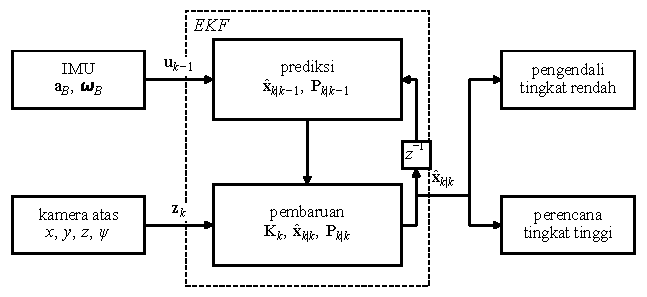
\includegraphics{figures/ekf.pdf}
    \caption{Fusi sensor dengan EKF. Prediksi dijalankan setiap cuplikan IMU; pembaruan dijalankan setiap pose kamera tiba. Estimasi $\hat{\mathbf{x}}_{k|k}$ diumpankan ke pengendali tingkat rendah dan perencana tingkat tinggi.}
    \label{fig:ekf_diagram}
\end{figure}

\subsection{Pengendali Tingkat Rendah}

Pengendali tingkat rendah berjalan pada \textit{flight controller} SpeedyBee F405 Mini (STM32F405) dengan \textit{firmware} ArduPilot Copter. Strukturnya kaskade: kalang translasi (posisi, kecepatan) di luar dan kalang rotasi (sikap, laju sudut) di dalam, seluruhnya ditutup oleh estimasi EKF3 (Gambar~\ref{fig:low_level_controller}). Tahapannya sebagai berikut.
\begin{enumerate}
    \item \textbf{Referensi gerak.} \textit{Companion computer} XIAO ESP32-S3 mengirim pesan MAVLink \texttt{SET\_}\allowbreak\texttt{POSITION\_}\allowbreak\texttt{TARGET\_}\allowbreak\texttt{LOCAL\_}\allowbreak\texttt{NED} melalui UART. Pesan memuat posisi acuan $\mathbf{p}_{\mathrm{ref}}$, kecepatan umpan-maju $\mathbf{v}_{\mathrm{ref}}$, dan sudut \textit{yaw} acuan $\psi_{\mathrm{ref}}$.
    \item \textbf{Kalang translasi.} Galat posisi $\mathbf{e}_p = \mathbf{p}_{\mathrm{ref}} - \hat{\mathbf{p}}$ diolah pengendali P posisi menjadi kecepatan komando $\mathbf{v}_{\mathrm{cmd}} = K_p^{\mathrm{pos}}\mathbf{e}_p$. Setelah ditambah $\mathbf{v}_{\mathrm{ref}}$ dan dibandingkan dengan $\hat{\mathbf{v}}$, pengendali PID kecepatan menghasilkan percepatan komando $\mathbf{a}_{\mathrm{cmd}}$.
    \item \textbf{Konversi akselerasi.} Dalam kerangka NED, besar gaya dorong adalah $T = m\,\lVert g\mathbf{e}_3 - \mathbf{a}_{\mathrm{cmd}} \rVert$ dengan $\mathbf{e}_3 = [0, 0, 1]^T$, dan arah vektor $g\mathbf{e}_3 - \mathbf{a}_{\mathrm{cmd}}$ bersama $\psi_{\mathrm{ref}}$ menentukan sikap target $\mathbf{q}_{\mathrm{des}}$ (\textit{quaternion}).
    \item \textbf{Kalang rotasi.} Galat antara $\mathbf{q}_{\mathrm{des}}$ dan $\hat{\mathbf{q}}$ diolah pengendali P sikap menjadi laju sudut target $\boldsymbol{\omega}_{\mathrm{des}}$; pengendali PID laju sudut membandingkannya dengan $\hat{\boldsymbol{\omega}}$ dan menghasilkan torsi komando $\boldsymbol{\tau} = [\tau_\phi, \tau_\theta, \tau_\psi]^T$.
    \item \textbf{Alokasi motor.} \textit{Mixer} memetakan $T$ dan $\boldsymbol{\tau}$ ke komando empat motor sesuai konfigurasi X, dikirim dengan protokol digital DShot ke ESC 4-in-1 SpeedyBee BLS 35A.
    \item \textbf{Estimasi.} EKF3 memadukan IMU ICM-42688P dengan pose kamera yang diterima sebagai \textit{external navigation} melalui MAVLink, menghasilkan $\hat{\mathbf{p}}$, $\hat{\mathbf{v}}$, $\hat{\mathbf{q}}$, dan $\hat{\boldsymbol{\omega}}$ untuk kedua kalang.
\end{enumerate}

\begin{figure}[htbp]
    \centering
    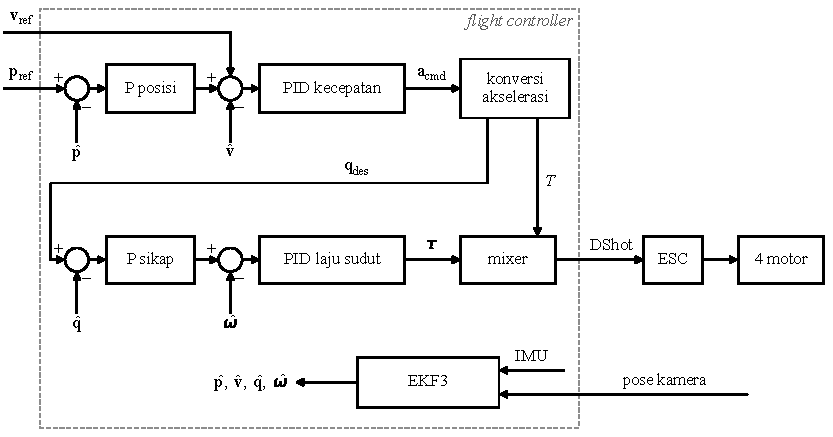
\includegraphics{figures/pengendali.pdf}
    \caption[Pengendali tingkat rendah kaskade pada \textit{flight controller}.]{Pengendali tingkat rendah kaskade pada \textit{flight controller}. Garis putus membatasi komputasi di dalam \textit{flight controller}; pose kamera datang dari \textit{companion computer}.}
    \label{fig:low_level_controller}
\end{figure}

\subsection{Perencana Tingkat Tinggi dan Formulasi ERC}
\label{subsec:erc}

Perencana tingkat tinggi dijalankan terpisah pada \textit{companion computer} tiap agen. Keluarannya berupa kecepatan acuan yang diintegrasikan menjadi \textit{setpoint} posisi bagi pengendali tingkat rendah (Gambar~\ref{fig:high_level_planner}). Formulasi berikut mengikuti rancangan penelitian sebelumnya \cite{herdianDecentralizedFormationControl2026, PerancanganSistemKendali}, yang mengembangkan ERC dari Bui \textit{et al.} \cite{buiEventbasedReconfigurationControl2025}, dan sesuai dengan implementasi simulator yang digunakan.

\begin{figure}[htbp]
    \centering
    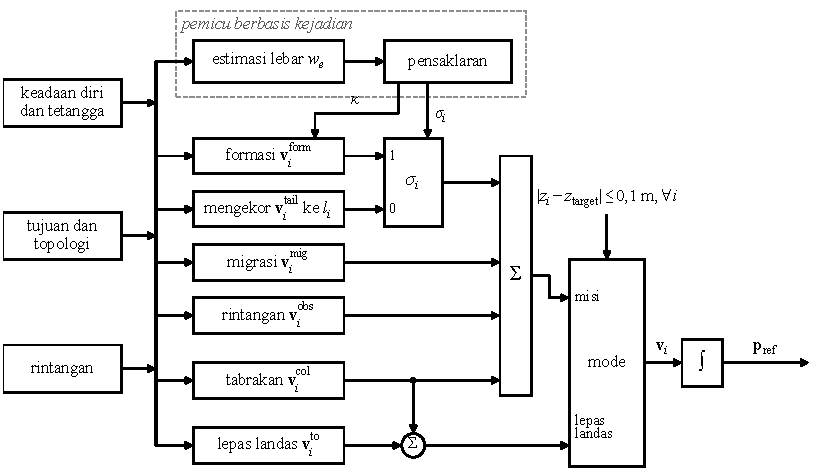
\includegraphics{figures/perencana.pdf}
    \caption[Perencana tingkat tinggi pada tiap agen.]{Perencana tingkat tinggi pada tiap agen, diadaptasi dari \cite{herdianDecentralizedFormationControl2026}. Lebar ruang $w_e$ menentukan faktor skala $\kappa$ dan mode $\sigma_i$ (Persamaan~\ref{eq:erc_pemicu}); kecepatan $\mathbf{v}_i$ diintegrasikan menjadi $\mathbf{p}_{\mathrm{ref}}$ bagi pengendali tingkat rendah.}
    \label{fig:high_level_planner}
\end{figure}

\subsubsection{Mode Misi}

Setiap agen berada pada salah satu dari tiga mode. Pada mode lepas landas, hanya perilaku lepas landas dan penghindaran tabrakan antaragen yang aktif; seluruh agen beralih bersamaan ke mode misi setelah $|z_i - z_{\mathrm{target}}| \le 0{,}1$~m untuk semua $i$. Pada mode misi, kecepatan acuan agen ke-$i$ adalah
\begin{equation}
    \mathbf{v}_i = \mathbf{v}_i^{\mathrm{mig}} + \mathbf{v}_i^{\mathrm{obs}} + \mathbf{v}_i^{\mathrm{col}} + \sigma_i\,\mathbf{v}_i^{\mathrm{form}} + (1-\sigma_i)\,\mathbf{v}_i^{\mathrm{tail}}
    \label{eq:erc_kecepatan}
\end{equation}
dengan $\sigma_i = 1$ pada mode formasi dan $\sigma_i = 0$ pada mode mengekor.

\subsubsection{Perilaku Penyusun}

Perilaku migrasi mengarahkan kawanan ke tujuan $\mathbf{p}_g$ dari pusat kawanan $\bar{\mathbf{p}}$ dengan laju acuan $V_{\mathrm{ref}}$:
\begin{equation}
    \mathbf{v}_i^{\mathrm{mig}} = V_{\mathrm{ref}}\,\frac{\mathbf{p}_g - \bar{\mathbf{p}}}{\lVert \mathbf{p}_g - \bar{\mathbf{p}} \rVert}
\end{equation}

Perilaku formasi menjaga posisi relatif terhadap topologi nominal $\boldsymbol{\delta}^*$ yang dirotasi searah lintasan, diskalakan oleh faktor $\kappa$:
\begin{equation}
    \mathbf{v}_i^{\mathrm{form}} = W_{\mathrm{form}} \sum_{j \neq i} \left[ (\mathbf{p}_j - \mathbf{p}_i) - \kappa\,(\boldsymbol{\delta}_j^* - \boldsymbol{\delta}_i^*) \right]
    \label{eq:erc_formasi}
\end{equation}

Penghindaran rintangan dan tabrakan antaragen berbentuk medan potensial tolak yang aktif di dalam radius waspada $R_a$, dengan $d$ jarak ke titik rintangan terdekat atau ke agen lain dan $\hat{\mathbf{n}}$ vektor satuan yang menjauhinya:
\begin{align}
    \mathbf{v}_i^{\mathrm{obs}} &= W_{\mathrm{obs}} \sum_{d_{io} < R_a} 0{,}5 \left( \frac{1}{d_{io}} - \frac{1}{R_a} \right) \frac{\hat{\mathbf{n}}_{io}}{d_{io}^2} \\
    \mathbf{v}_i^{\mathrm{col}} &= W_{\mathrm{col}} \sum_{d_{ij} < R_a} 2 \left( \frac{1}{d_{ij}} - \frac{1}{R_a} \right) \frac{\hat{\mathbf{n}}_{ij}}{d_{ij}^2}
\end{align}

Pada mode mengekor, agen mengikuti pemimpin lokal $l$ pada jarak acuan $d_{\mathrm{ref}}$ searah kecepatan pemimpin $\hat{\mathbf{u}}_l$:
\begin{equation}
    \mathbf{v}_i^{\mathrm{tail}} = W_{\mathrm{tail}} \left[ (\mathbf{p}_l - \mathbf{p}_i - d_{\mathrm{ref}}\,\hat{\mathbf{u}}_l) + \mathbf{v}_l \right]
\end{equation}

\subsubsection{Pemicu Berbasis Kejadian}

Lebar ruang bebas $w_e$ diperoleh dari titik rintangan terdekat di sisi kiri $\mathbf{o}_l$ dan kanan $\mathbf{o}_r$ yang berada di depan agen, diproyeksikan ke sumbu tegak lurus arah gerak $\mathbf{u}_{\mathrm{ref}}^{\perp}$:
\begin{equation}
    w_e = \left| \left\langle \mathbf{o}_r - \mathbf{o}_l,\; \mathbf{u}_{\mathrm{ref}}^{\perp} \right\rangle \right|
\end{equation}
Nilai $w_e$ menentukan mode dan faktor skala formasi:
\begin{equation}
    (\sigma_i, \kappa) =
    \begin{cases}
        (0,\ \text{--}), & w_e \le \alpha R \\[2pt]
        \left(1,\ \min\left\{1,\ \dfrac{w_e - 2R}{w_f}\right\}\right), & w_e > \alpha R
    \end{cases}
    \label{eq:erc_pemicu}
\end{equation}
dengan $R$ jari-jari agen, $\alpha$ faktor ambang, dan $w_f$ bentang lateral nominal formasi. Bila tidak ada rintangan di kedua sisi, $\sigma_i = 1$ dan $\kappa = 1$. Dengan demikian formasi menyusut proporsional saat lorong menyempit dan baru beralih mengekor ketika $w_e$ melewati ambang $\alpha R$. Tidak ada pita histeresis pada perpindahan mode.

Saat beralih ke mode mengekor, setiap agen memilih pemimpinnya secara terdesentralisasi, yaitu agen terdekat yang berada di depannya sepanjang arah menuju tujuan $\hat{\mathbf{g}}$:
\begin{equation}
    l_i = \arg\min_{j\,:\,p_{ij} > 0} p_{ij}, \qquad p_{ij} = \langle \mathbf{p}_j - \mathbf{p}_i,\ \hat{\mathbf{g}} \rangle
\end{equation}
Agen tanpa agen lain di depannya menjadi pemimpin barisan.

Pada versi simulator yang digunakan (\texttt{0d7ed5a}), nilai $\kappa$ pada Persamaan~\ref{eq:erc_pemicu} telah dihitung dan dicatat, tetapi belum diterapkan pada perilaku formasi Persamaan~\ref{eq:erc_formasi}. Penerapannya beserta pengulangan skenario lorong sempit dijadwalkan pada Fase~1.

\subsubsection{Parameter}

Nilai parameter pada Tabel~\ref{tab:parameter_erc} merupakan nilai simulasi dan akan disetel ulang untuk wahana fisik. Untuk wahana berjari-jari efektif $R = 0{,}125$~m, ambang mengekor menjadi $\alpha R = 1{,}0$~m, sehingga celah arena selebar $0{,}90$~m memicu mode mengekor sedangkan koridor terbuka selebar $2{,}70$~m mempertahankan formasi. Berbeda dengan simulasi yang menghitung $w_e$ dari peta rintangan, pada wahana fisik $w_e$ diestimasi dari pembacaan sensor jarak lateral (Gambar~\ref{fig:ultrasonic_placement}).

\begin{table}[htbp]
    \centering
    \caption{Parameter perencana tingkat tinggi pada simulasi}
    \label{tab:parameter_erc}
    \begingroup
    \small
    \renewcommand{\arraystretch}{1.25}
    \begin{tabularx}{\textwidth}{|X|>{\centering\arraybackslash}p{2.0cm}|>{\centering\arraybackslash}p{2.4cm}|}
        \hline
        \rowcolor{gray!20}
        \thead{Parameter} & \thead{Simbol} & \thead{Nilai} \\ \hline
        Jari-jari agen & $R$ & $0{,}2$ m \\ \hline
        Faktor ambang mengekor & $\alpha$ & $8$ \\ \hline
        Radius waspada & $R_a = 3R$ & $0{,}6$ m \\ \hline
        Bentang lateral nominal formasi & $w_f$ & $2{,}0$ m \\ \hline
        Laju acuan migrasi & $V_{\mathrm{ref}}$ & $0{,}5$ m/s \\ \hline
        Jarak acuan mengekor & $d_{\mathrm{ref}}$ & $1{,}0$ m \\ \hline
        Bobot formasi & $W_{\mathrm{form}}$ & $1{,}0$ \\ \hline
        Bobot mengekor & $W_{\mathrm{tail}}$ & $1{,}2$ \\ \hline
        Bobot rintangan dan tabrakan & $W_{\mathrm{obs}},\ W_{\mathrm{col}}$ & $8{,}0$ \\ \hline
    \end{tabularx}
    \endgroup
\end{table}

\section{Rancangan Arena Uji}
\label{sec:arena}

Arena dirancang agar peristiwa pemicu rekonfigurasi benar-benar muncul karena penyempitan ruang yang dirancang, bukan karena keterbatasan arena itu sendiri. Rancangannya diturunkan dengan menskalakan geometri yang telah divalidasi pada simulasi \cite{herdianDecentralizedFormationControl2026} ke dimensi wahana dan ruang yang tersedia.

Pada simulasi, agen dimodelkan berdiameter $0{,}40$ m dengan topologi formasi V berbentang lateral $2{,}40$ m, melintasi lorong sempit selebar $1{,}00$ m. Dua perbandingan menentukan perilaku sistem: bentang formasi terhadap lebar celah, dan lebar celah terhadap diameter agen. Perbandingan pertama menentukan apakah peristiwa pemicu muncul sama sekali, sedangkan perbandingan kedua menentukan seberapa ketat manuver mengekor harus dilakukan. Penskalaan mempertahankan perbandingan tersebut, bukan nilai mutlaknya.

Dengan lebar bersih koridor $270$ cm dan syarat ruang bebas sekurang-kurangnya $30$ cm pada tiap sisi, bentang formasi maksimum yang dapat diuji adalah $205$ cm, yang tercapai pada faktor skala $0{,}9$. Lebar celah mengikuti pada $90$ cm. Perbandingan hasil penskalaan terhadap nilai pada simulasi dirangkum pada Tabel~\ref{tab:penskalaan_arena}.

\begin{table}[htbp]
    \centering
    \caption{Penskalaan geometri skenario dari simulasi ke arena fisik}
    \label{tab:penskalaan_arena}
    \begingroup
    \small
    \renewcommand{\arraystretch}{1.3}
    \begin{tabularx}{\textwidth}{|X|>{\centering\arraybackslash}p{2.6cm}|>{\centering\arraybackslash}p{2.6cm}|}
        \hline
        \rowcolor{gray!20}
        \thead{Besaran} & \thead{Simulasi} & \thead{Arena fisik} \\ \hline
        Diameter agen & $0{,}40$ m & $0{,}25$ m \\ \hline
        Bentang lateral formasi & $2{,}40$ m & $2{,}05$ m \\ \hline
        Lebar celah & $1{,}00$ m & $0{,}90$ m \\ \hline
        Panjang bagian sempit & $5{,}00$ m & $1{,}80$ m \\ \hline
        Rasio bentang formasi terhadap celah & $2{,}40$ & $2{,}28$ \\ \hline
        Rasio celah terhadap diameter agen & $2{,}50$ & $3{,}60$ \\ \hline
    \end{tabularx}
    \endgroup
\end{table}

Dua perbedaan pada Tabel~\ref{tab:penskalaan_arena} memengaruhi penafsiran hasil. Pertama, rasio celah terhadap diameter agen di arena lebih besar karena wahana nyata relatif lebih ramping, sehingga keberhasilan di arena tidak serta-merta membuktikan keberhasilan pada rasio simulasi yang lebih ketat. Kedua, bagian sempit arena hanya $1{,}80$ m sehingga fase mengekor lebih singkat. Untuk perbedaan kedua, simulator diberi skema baru yang meniru geometri arena, bukan arena yang dipaksa meniru simulasi.

Tata letak arena selengkapnya diperlihatkan pada Gambar~\ref{fig:sketsa_arena}. Salah satu kolom bangunan yang menjorok ke koridor menjadi satu sisi penyempitan karena posisinya permanen, sehingga geometri rintangan dapat direproduksi antarsesi tanpa pengukuran ulang. Sisi seberangnya dilengkapi susunan dus kardus yang menjorok sedalam $1{,}01$ m sehingga menyisakan celah $90$ cm.

\begin{figure}[htbp]
    \centering
    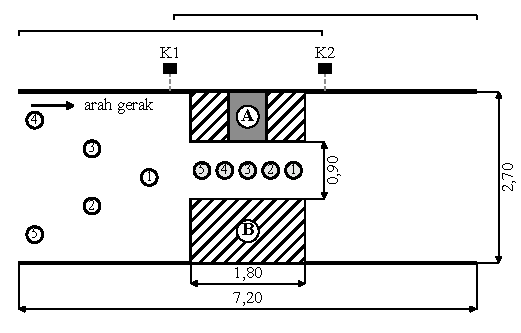
\includegraphics{figures/arena.pdf}
    \caption{Denah arena uji (satuan m). A: kolom bangunan $0{,}60 \times 0{,}79$~m; B: dus rintangan. Lingkaran putih menunjukkan formasi V saat mendekat dan lingkaran abu-abu formasi mengekor di dalam kanal, dengan agen 1 memimpin. K1 dan K2 adalah posisi kamera; kurung di atas denah menunjukkan liputan minimum masing-masing kamera.}
    \label{fig:sketsa_arena}
\end{figure}

Pada konfigurasi ini, wahana menyisakan ruang bebas $32{,}5$ cm pada tiap sisi baik saat mempertahankan formasi V di koridor terbuka maupun saat mengekor melewati celah. Margin yang seragam tersebut dipilih agar tuntutan ketelitian kendali pada kedua fase manuver setara, sehingga kegagalan pada salah satu fase dapat ditafsirkan sebagai persoalan algoritma dan bukan sekadar akibat arena yang terlalu sempit pada fase tersebut.

\section{Arsitektur Sistem Menyeluruh}
\label{sec:arsitektur_sistem}

Keseluruhan subsistem yang telah diuraikan disatukan ke dalam arsitektur pada Gambar~\ref{fig:arsitektur_sistem}. Aliran data bermula dari dua kamera atas yang mengamati penanda visual pada tiap wahana. Stasiun pemroses citra di darat menjalankan deteksi penanda dan penyelesaian \textit{Perspective-n-Point} untuk menghasilkan pose tiga dimensi kelima agen, lalu menyiarkannya melalui jaringan Wi-Fi lokal berbasis soket UDP. Pada tiap wahana, \textit{companion computer} menerima pose tersebut, memadukannya dengan pembacaan sensor jarak, menjalankan algoritma IAPF dan ERC, lalu meneruskan \textit{setpoint} posisi ke \textit{flight controller} melalui antarmuka serial berformat MAVLink. \textit{Flight controller} menutup kalang kendali hingga alokasi perintah motor.

\begin{figure}[htbp]
    \centering
    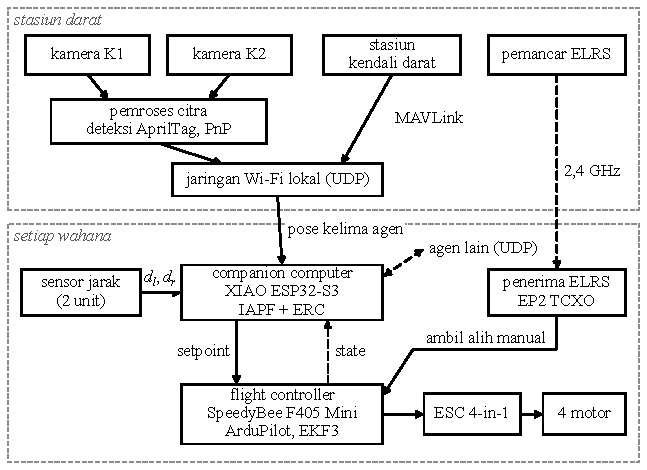
\includegraphics{figures/arsitektur-sistem.pdf}
    \caption{Arsitektur sistem. Garis penuh menunjukkan aliran data utama; garis putus menunjukkan umpan balik \textit{state}, komunikasi antarwahana, dan tautan radio ELRS 2,4~GHz yang menjadi jalur pengambilalihan manual tanpa bergantung pada jaringan Wi-Fi.}
    \label{fig:arsitektur_sistem}
\end{figure}

Arsitektur ini memisahkan \textbf{lokalisasi} (kamera atas) dari \textbf{persepsi} (sensor jarak pada wahana). Karena rintangan statis dan posisinya diketahui, $w_e$ sebenarnya dapat dihitung terpusat dari kamera lalu disiarkan. Hal itu tidak dilakukan: agen yang membaca peta kiriman pusat tidak lagi mempersepsi lingkungannya sendiri, dan sifat terdesentralisasi yang melandasi ERC gugur.

% ==========================================
% BAB IV METODOLOGI DAN RENCANA PELAKSANAAN
% ==========================================
\chapter{METODOLOGI DAN RENCANA PELAKSANAAN}

\section{Kerangka Metodologi}

Penelitian dibagi ke dalam lima fase (Gambar~\ref{fig:diagram_metodologi}). Tiga titik keputusan menjadi gerbang kelayakan: evaluasi HITL pada Fase~3, kestabilan wahana tunggal, dan keberhasilan misi kawanan pada Fase~4. Bila gerbang tidak terlewati, pekerjaan kembali ke penanaman logika, bukan ke awal penelitian.

Pengadaan mengikuti gerbang tersebut. Komponen untuk lima wahana baru dibeli setelah uji terbang tunggal lolos, karena tiga ketidakpastian hanya dapat dijawab melalui percobaan: apakah \textit{firmware} racikan muat pada memori \textit{flash} 1~MB (Subbab~\ref{subsec:firmware_fc}), apakah penanda terdeteksi andal saat wahana bergerak (Subbab~\ref{subsec:liputan_kamera}), dan sensor jarak mana yang andal pada sudut datang miring (Subbab~\ref{subsec:pemilihan_sensor}).

\begin{figure}[htbp]
    \centering
    
\includegraphics[width=\textwidth]{figures/metodologi_tesis.pdf}
    \caption{Diagram alir metodologi penelitian.}
    \label{fig:diagram_metodologi}
\end{figure}

\section{Fase 1: Studi dan Desain Arsitektur}

\begin{enumerate}
    \item \textbf{Studi literatur} dinamika quadcopter dan evaluasi simulasi ERC, berlangsung sepanjang penelitian. Termasuk di dalamnya penerapan faktor skala $\kappa$ pada simulator (Subbab~\ref{subsec:erc}) dan simulasi arena berskala dengan geometri Tabel~\ref{tab:penskalaan_arena}, yang hasilnya menjadi pembanding pada Fase~5.
    \item \textbf{Desain arsitektur} lima quadcopter dengan pembagian kerja antara \textit{flight controller} sebagai pengendali tingkat rendah dan \textit{companion computer} sebagai perencana tingkat tinggi (Bab~III).
\end{enumerate}
Fase ini tidak memerlukan pengadaan.

\section{Fase 2: Implementasi Teknologi}

\begin{enumerate}
    \item \textbf{Komunikasi internal.} \textit{Firmware} ArduPilot racikan dibangun (Subbab~\ref{subsec:firmware_fc}), lalu antarmuka UART MAVLink antara \textit{companion computer} dan \textit{flight controller} dikonfigurasi.
    \item \textbf{Komunikasi eksternal.} Jaringan terdesentralisasi antaragen dibangun dengan UDP melalui Wi-Fi.
    \item \textbf{Lokalisasi.} Kamera pertama dikalibrasi; deteksi penanda AprilTag, penyelesaian pose, pengiriman MAVLink, dan fusi EKF dijalankan menerus. Pada tahap ini pula HC-SR04 dan VL53L1X diuji banding dengan kriteria pada Subbab~\ref{subsec:pemilihan_sensor}.
    \item \textbf{Penanaman logika} algoritma ERC dan IAPF pada \textit{companion computer}.
    \item \textbf{Tautan kendali manual.} Pemancar ExpressLRS diikat ke penerima EP2 TCXO yang telah tersedia. Pemancar diadakan sebelum uji terbang karena merupakan satu-satunya jalur penghentian darurat yang tidak bergantung pada Wi-Fi.
\end{enumerate}

\begin{table}[htbp]
    \centering
    \caption{Anggaran Fase 2}
    \label{tab:rab_fase2}
    \begingroup
    \small
    \setlength{\tabcolsep}{3pt}
    \renewcommand{\arraystretch}{1.3}
    \begin{tabularx}{\textwidth}{|c|X|>{\centering\arraybackslash}p{1.35cm}|>{\raggedleft\arraybackslash}p{2.1cm}|>{\raggedleft\arraybackslash}p{2.8cm}|}
        \hline
        \rowcolor{gray!20}
        \thead{No} & \thead{Komponen} & \thead{Jumlah} & \thead{Harga\\Satuan (Rp)} & \thead{Harga\\Total (Rp)} \\ \hline
        1 & Kamera USB 5 MP \textit{global shutter}, lensa $120^\circ$ & 1 unit & \textit{survei} & \textit{survei} \\ \hline
        2 & Kabel USB ekstensi 10 m dan dudukan langit-langit & 1 set & 150.000 & 150.000 \\ \hline
        3 & Pemancar ExpressLRS 2,4 GHz RadioMaster Pocket & 1 unit & 1.150.000 & 1.150.000 \\ \hline
        4 & Sensor ultrasonik HC-SR04 (kandidat) & 2 unit & 20.000 & 40.000 \\ \hline
        5 & Sensor jarak laser VL53L1X (kandidat) & 2 unit & \textit{survei} & \textit{survei} \\ \hline
        6 & Penanda AprilTag, akrilik, dan tiang cetak tiga dimensi & 1 set & 20.000 & 20.000 \\ \hline
        \multicolumn{4}{|r|}{\textbf{Subtotal}} & \textbf{1.360.000 + \textit{survei}} \\ \hline
    \end{tabularx}
    \endgroup
\end{table}

\section{Fase 3: Pengujian \textit{Hardware-in-the-Loop}}

Algoritma pada \textit{companion computer} dijalankan dengan umpan balik simulasi gerak untuk mengukur beban CPU dan latensi komputasi sebelum wahana diterbangkan. Fase ini tidak memerlukan pengadaan.

\noindent\textbf{Gerbang Fase 3:} beban CPU dan latensi berada dalam batas aman. Bila terjadi tunda atau galat program, pekerjaan kembali ke penanaman logika.

\section{Fase 4: Uji Terbang Eksperimen}

\begin{enumerate}
    \item \textbf{Uji terbang tunggal.} Satu quadcopter memvalidasi EKF, tautan \textit{companion computer} ke \textit{flight controller}, penalaan PID, dan logika ERC agen tunggal. Deteksi penanda saat wahana bergerak dan jenis sensor jarak terpilih ikut dipastikan pada tahap ini.

    \noindent\textbf{Gerbang:} wahana tunggal stabil dan aman.

    \item \textbf{Uji terbang kawanan.} Kamera kedua dipasang dan kedua kamera dikalibrasi ke satu kerangka acuan global. Inventaris (Tabel~\ref{tab:komponen_tersedia}) memuat empat \textit{flight controller} dan ESC serta satu \textit{companion computer}, sehingga kekurangannya dilengkapi pada tahap ini. Kelima wahana lebih dahulu terbang dalam formasi V di ruang terbuka sebagai acuan, kemudian melintasi arena (Subbab~\ref{sec:arena}): lebar ruang $w_e$ yang turun melewati ambang memicu ERC sehingga formasi menyusut, beralih mengekor melalui celah $90$~cm, lalu mengembang kembali.

    \noindent\textbf{Gerbang:} manuver kawanan berhasil dan stabil.
\end{enumerate}

\begin{table}[htbp]
    \centering
    \caption{Anggaran Fase 4}
    \label{tab:rab_fase4}
    \begingroup
    \small
    \setlength{\tabcolsep}{3pt}
    \renewcommand{\arraystretch}{1.3}
    \begin{tabularx}{\textwidth}{|c|X|>{\centering\arraybackslash}p{1.35cm}|>{\raggedleft\arraybackslash}p{2.1cm}|>{\raggedleft\arraybackslash}p{2.8cm}|}
        \hline
        \rowcolor{gray!20}
        \thead{No} & \thead{Komponen} & \thead{Jumlah} & \thead{Harga\\Satuan (Rp)} & \thead{Harga\\Total (Rp)} \\ \hline
        \multicolumn{5}{|l|}{\textit{Sebelum uji terbang tunggal}} \\ \hline
        1 & Perlengkapan keselamatan (tas tahan api baterai, jaring, kacamata) & 1 set & 500.000 & 500.000 \\ \hline
        \multicolumn{5}{|l|}{\textit{Setelah uji terbang tunggal lolos}} \\ \hline
        2 & Kamera USB 5 MP \textit{global shutter} kedua, lensa $120^\circ$ & 1 unit & \textit{survei} & \textit{survei} \\ \hline
        3 & Kabel USB ekstensi 10 m dan dudukan langit-langit & 1 set & 150.000 & 150.000 \\ \hline
        4 & Sensor jarak terpilih & 8 unit & \textit{survei} & \textit{survei} \\ \hline
        5 & Penanda AprilTag, akrilik, dan tiang cetak tiga dimensi & 4 set & 20.000 & 80.000 \\ \hline
        6 & Penerima ExpressLRS EP2 TCXO & 2 unit & 215.000 & 430.000 \\ \hline
        7 & \textit{Stack} SpeedyBee F405 Mini dan ESC BLS 35A & 1 set & 1.906.700 & 1.906.700 \\ \hline
        8 & \textit{Companion computer} Seeed XIAO ESP32-S3 & 4 unit & 198.000 & 792.000 \\ \hline
        9 & Dus kardus sebagai rintangan & 10 unit & 30.000 & 300.000 \\ \hline
        10 & Lakban penanda posisi lantai & 1 set & \textit{survei} & \textit{survei} \\ \hline
        \multicolumn{4}{|r|}{\textbf{Subtotal}} & \textbf{4.158.700 + \textit{survei}} \\ \hline
    \end{tabularx}
    \endgroup
\end{table}

Harga sensor jarak mengikuti hasil uji banding; bila HC-SR04 terpilih, pos tersebut bernilai Rp160.000.

\section{Fase 5: Analisis Data dan Pelaporan}

Data diekstraksi dari \textit{log} pose EKF, riwayat pemicu ERC, dan trafik UDP. Metrik yang dihitung adalah RMSE galat formasi, waktu konvergensi, tingkat keberhasilan melintasi celah, jarak minimum antaragen, serta beban komputasi dan \textit{bandwidth}. Hasil fisik dibandingkan dengan simulasi arena berskala dari Fase~1, lalu disusun menjadi tesis dan naskah publikasi. Fase ini tidak memerlukan pengadaan.

\section{Rencana Pelaksanaan}

\subsection{Lokasi}
Seluruh kegiatan berlangsung di Pusat Teknologi Instrumentasi dan Otomasi (PTIO\label{abbr:ptio}) ITB, Gedung Pusat Antar Universitas Lantai~8. Uji terbang dilakukan di koridor yang diuraikan pada Subbab~\ref{subsec:kondisi_ruang}.

\subsection{Rekapitulasi Anggaran}
\label{subsec:rab}

Rencana Anggaran Biaya (RAB\label{abbr:rab}) dirangkum pada Tabel~\ref{tab:rekap_rab}. Harga bersumber dari RAB awal penulis dan survei Tokopedia pada September 2026; pos bertanda \textit{survei} belum memiliki harga dan tidak diperkirakan.

\begin{table}[htbp]
    \centering
    \caption{Rekapitulasi anggaran per fase}
    \label{tab:rekap_rab}
    \begingroup
    \small
    \renewcommand{\arraystretch}{1.3}
    \begin{tabularx}{\textwidth}{|l|>{\raggedleft\arraybackslash}p{3.0cm}|X|}
        \hline
        \rowcolor{gray!20}
        \thead{Fase} & \thead{Harga pasti (Rp)} & \thead{Pos menunggu survei} \\ \hline
        Fase 1: Studi dan Desain Arsitektur & -- & -- \\ \hline
        Fase 2: Implementasi Teknologi & 1.360.000 & kamera, VL53L1X \\ \hline
        Fase 3: Pengujian HITL & -- & -- \\ \hline
        Fase 4: Uji Terbang Eksperimen & 4.158.700 & kamera kedua, sensor jarak terpilih, lakban \\ \hline
        Fase 5: Analisis Data dan Pelaporan & -- & -- \\ \hline
        \textbf{Total} & \textbf{5.518.700} & \\ \hline
    \end{tabularx}
    \endgroup
\end{table}

\subsection{Jadwal Pelaksanaan}

Penelitian direncanakan selama sembilan bulan, dari September 2026 sampai Mei 2027, dengan rincian pada Tabel~\ref{tab:jadwal_pelaksanaan}. Bulan terakhir dikhususkan untuk ekstraksi data, analisis, dan penulisan.

\begin{table}[htbp]
    \centering
    \caption{Jadwal pelaksanaan penelitian September 2026--Mei 2027}
    \label{tab:jadwal_pelaksanaan}
    \renewcommand{\arraystretch}{1.3}
    \resizebox{\textwidth}{!}{%
    \begin{tabular}{|c|p{11.5cm}|c|c|c|c|c|c|c|c|c|}
        \hline
        \rowcolor{gray!20}
        & & \multicolumn{4}{c|}{\textbf{2026}} & \multicolumn{5}{c|}{\textbf{2027}} \\ \cline{3-11}
        \rowcolor{gray!20}
        \multirow{-2}{*}{\textbf{No}} & \multirow{-2}{=}{\centering\textbf{Kegiatan}} & \textbf{9} & \textbf{10} & \textbf{11} & \textbf{12} & \textbf{1} & \textbf{2} & \textbf{3} & \textbf{4} & \textbf{5} \\ \hline
        \multicolumn{11}{|l|}{\cellcolor{gray!10}\textbf{Fase 1: Studi dan Desain Arsitektur}} \\ \hline
        1 & Studi literatur: formasi multi-agen, dinamika wahana, dan simulasi ERC & \cellcolor{gray!70} & \cellcolor{gray!70} & \cellcolor{gray!70} & \cellcolor{gray!70} & \cellcolor{gray!70} & \cellcolor{gray!70} & \cellcolor{gray!70} & \cellcolor{gray!70} & \cellcolor{gray!70} \\ \hline
        2 & Desain arsitektur: lima quadcopter (\textit{flight controller} dan \textit{companion computer}) & \cellcolor{gray!70} &  &  &  &  &  &  &  &  \\ \hline
        \multicolumn{11}{|l|}{\cellcolor{gray!10}\textbf{Fase 2: Implementasi Teknologi}} \\ \hline
        3 & Komunikasi internal: \textit{firmware} racikan, antarmuka serial, dan \mbox{MAVLink}\label{abbr:mavlink} &  & \cellcolor{gray!70} & \cellcolor{gray!70} &  &  &  &  &  &  \\ \hline
        4 & Komunikasi eksternal: jaringan terdesentralisasi UDP\label{abbr:udp} &  & \cellcolor{gray!70} & \cellcolor{gray!70} &  &  &  &  &  &  \\ \hline
        5 & Lokalisasi kamera atas dan fusi EKF; uji banding sensor jarak &  & \cellcolor{gray!70} & \cellcolor{gray!70} &  &  &  &  &  &  \\ \hline
        6 & Penanaman logika: IAPF\label{abbr:iapf} dan ERC &  & \cellcolor{gray!70} & \cellcolor{gray!70} & \cellcolor{gray!70} &  &  &  &  &  \\ \hline
        \multicolumn{11}{|l|}{\cellcolor{gray!10}\textbf{Fase 3: Pengujian \textit{Hardware-in-the-Loop}}} \\ \hline
        7 & Uji HITL\label{abbr:hitl}: beban CPU dan latensi pada \textit{companion computer} &  &  &  & \cellcolor{gray!70} & \cellcolor{gray!70} &  &  &  &  \\ \hline
        \multicolumn{11}{|l|}{\cellcolor{gray!10}\textbf{Fase 4: Uji Terbang Eksperimen}} \\ \hline
        8 & Uji terbang tunggal: validasi EKF, tautan \textit{companion computer}--\textit{flight controller}, dan penalaan PID\label{abbr:pid} &  &  &  & \cellcolor{gray!70} & \cellcolor{gray!70} &  &  &  &  \\ \hline
        9 & Uji terbang kawanan: formasi V acuan di ruang terbuka &  &  &  &  & \cellcolor{gray!70} & \cellcolor{gray!70} &  &  &  \\ \hline
        10 & Uji terbang kawanan: formasi adaptif ERC melintasi celah $90$ cm &  &  &  &  &  & \cellcolor{gray!70} & \cellcolor{gray!70} & \cellcolor{gray!70} &  \\ \hline
        11 & Karakterisasi komunikasi: trafik UDP dan latensi &  &  &  &  &  &  & \cellcolor{gray!70} & \cellcolor{gray!70} &  \\ \hline
        \multicolumn{11}{|l|}{\cellcolor{gray!10}\textbf{Fase 5: Analisis Data dan Pelaporan}} \\ \hline
        12 & Ekstraksi data: log pose EKF, riwayat pemicu ERC, dan trafik UDP &  &  &  &  &  &  &  &  & \cellcolor{gray!70} \\ \hline
        13 & Analisis metrik: galat formasi (RMSE\label{abbr:rmse}), keberhasilan melintasi celah, dan beban komunikasi &  &  &  &  &  &  &  &  & \cellcolor{gray!70} \\ \hline
        14 & Penyusunan tesis dan naskah publikasi &  &  &  &  &  &  &  &  & \cellcolor{gray!70} \\ \hline
    \end{tabular}%
    }
\end{table}

% ==========================================
% BAB V PENUTUP
% ==========================================
\chapter{PENUTUP}
Dokumen proposal tesis ini telah memaparkan landasan teoretis, pertimbangan teknis, serta rencana implementasi fisik dan evaluasi sistem kontrol formasi terdesentralisasi berbasis \textit{Event-Based Reconfiguration Control} (ERC) pada kawanan lima unit \textit{quadcopter} di ruang sempit. Melalui pendekatan bertahap yang diawali dengan pembuktian jalur kerja pada satu wahana hingga uji skala penuh kawanan, penelitian ini dirancang untuk menjawab kesenjangan antara simulasi numerik dan keterbatasan fisik dunia nyata. 

Luaran utama yang ditargetkan dari penelitian ini meliputi: (1) arsitektur sistem perangkat keras dan perangkat lunak terdesentralisasi yang siap direplikasi, (2) pustaka program algoritma ERC dan IAPF yang teruji pada sistem tertanam, (3) dataset penerbangan eksperimental yang memvalidasi efisiensi \textit{bandwidth} dan akurasi pelacakan posisi secara empiris, serta (4) naskah tesis magister dan publikasi ilmiah pada jurnal atau konferensi terindeks bereputasi. Dengan mitigasi risiko teknis melalui mekanisme pengambilalihan manual radio independen dan gerbang kelayakan bertahap, diharapkan penelitian ini dapat terlaksana sesuai dengan jadwal dan memberikan kontribusi nyata bagi pengembangan sistem robotika kawanan otonom.

% ==========================================
% DAFTAR PUSTAKA (MENGGUNAKAN BERKAS EKSTERNAL)
% ==========================================
\clearpage
\renewcommand{\bibname}{DAFTAR PUSTAKA} % Mengubah judul bawaan menjadi "DAFTAR PUSTAKA".
\addcontentsline{toc}{chapter}{DAFTAR PUSTAKA} % Memasukkan daftar pustaka ke dalam daftar isi.

% Menentukan gaya tampilan daftar pustaka.
\bibliographystyle{IEEEtranN}

% Memuat basis data pustaka dari berkas references.bib.
\bibliography{../common/references}

\end{document}